\externaldocument{Introduction.tex}
\externaldocument{Experimental_Apparatus.tex}
\externaldocument{Results.tex}
\externaldocument{Analysis.tex}
\externaldocument{Checks_and_Systematics.tex}
% \externaldocument{EIC_Jets.tex}
\externaldocument{Discussion.tex}
\chapter{The Electron Ion Collider}
The Electron Ion Collider (EIC) is a planned US-based facility that will make precision measurements of the collisions of electrons with polarized protons 
%bvj and light ions, as well as heavy ions, 
and ions over a large mass range
%
to study Quantum Chromodynamics (QCD) \cite{Accardi:2012qut,Aschenauer:2017jsk}. Electrons with energies up to 18 GeV will collide with protons up to 275 GeV and ions with energies up to 110 GeV per nucleon, at luminosities up to $10^{34}$ cm$^{-2}$ s$^{-1}$~\cite{eRHIC:preCDR}. The EIC will explore a very wide range of physics topics, including - among others - the spin structure of protons and light nuclei, the partonic structure of light and heavy ions, parton transport in nuclear matter, and the hadronization process. The analysis in this chapter will primarily focus on the latter two topics using jets to study the fragmentation functions as the parton transport in the nucleus. 


\begin{figure}[htpb]
  \centering
  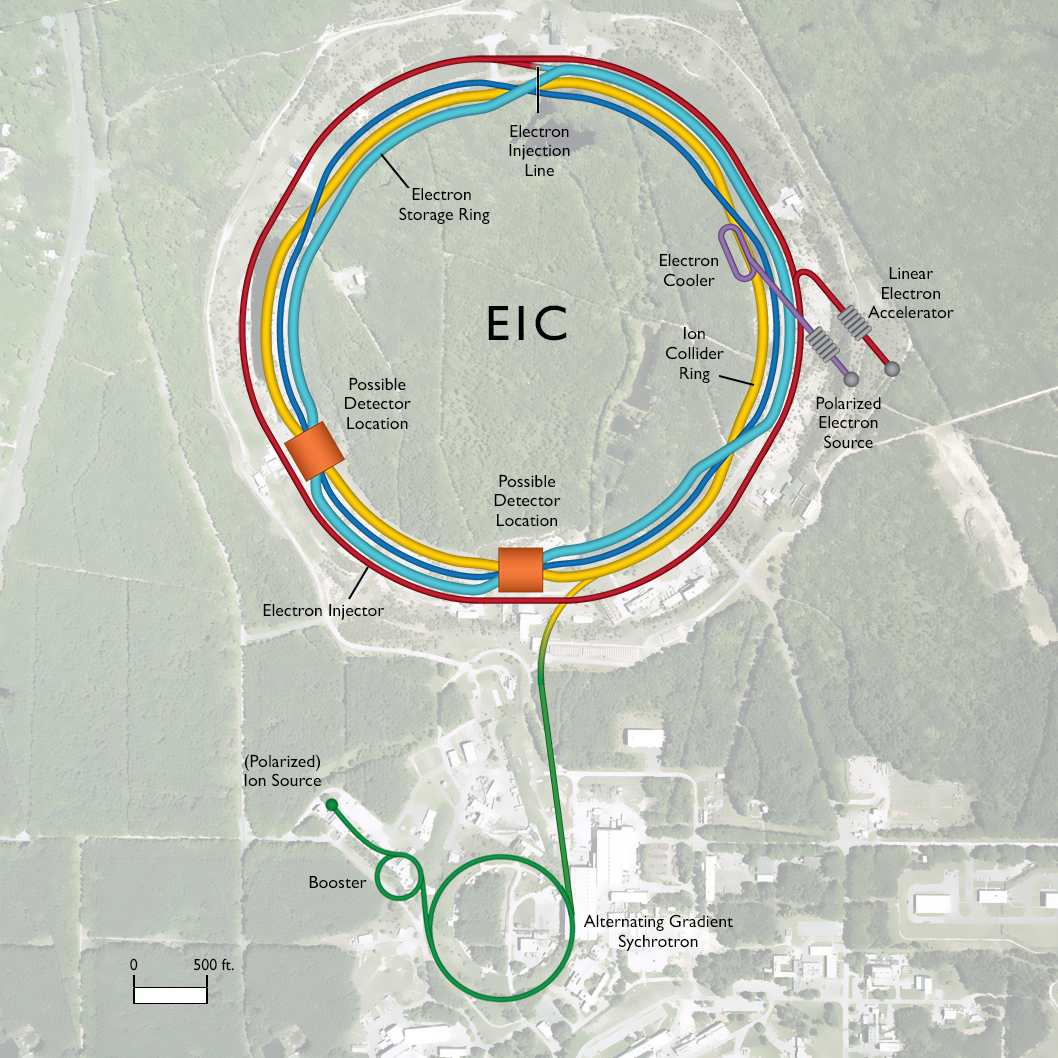
\includegraphics[width=0.8\textwidth]{EIC_Jets/eic.jpg}
  \caption{Schematic of how the EIC will fit within the tunnel of the Relativistic Heavy Ion Collider reusing essential infrastructure and key components of RHIC \cite{zotero-283}.}
  \label{fig:eic}
\end{figure}

The ALICE $\gamma$-hadron measurements in this dissertation constrain the modification of the parton fragmentation function due to cold nuclear matter effects within 13\% for a  $x_\mathrm{T}$ range of approximately $0.005-0.016$. But despite ALICE being  $the$ heavy-ion detector at the LHC, the large particle multiplicities and high energies make precise measurements of  $Q^2$ impossible, ruling out comparisons to many theoretical models of cold nuclear matter effects. The EIC, however, makes measurements of $Q^2$ trivial; the EIC was designed from the ground up for that very purpose. Studying the charged jet fragmentation function at the EIC can place much tighter constraints on modifications to the fragmentation function. Additionally, measurements of electron-jet correlations can probe the mean energy of a parton lost to the nucleus, $\hat{q}L$. 

While the $\gamma$-hadron correlations place very important constraints on cold nuclear matter effects, it does so as a small part of general-purpose detector with a very large heavy-ion program, largely focused on the development of the quark gluon plasma. Jet measurements at the EIC however, can probe the nucleus much more precisely through semi-inclusive deep inelastic scattering and furthermore help quantify certain properties of the nucleus. This chapter focuses on such measurements, done with a novel all-silicon tracker design for the EIC. The tracker will be described in detail, followed by a description of the simulated jet reconstruction performance, and end with the simulation of two physical observables to be measured at the EIC.

% \section{All-Sillicon Tracker}
% \section{Analysis}
% \subsection{Simulation}
% \subsection{NTuples}
% \subsection{Jet Reconstruction}
% \subsection{Electron Smearing}
% \subsection{Luminosity Scaling}
% \section{Results}
% \subsection{Electron-Jet Correlations}
% \subsection{Charged Jet Fragmentation Function}
% \section{Conclusion}

\section{All-Silicon Tracker Concept Design}
\label{sec:sim:full}

% \section{Requirements on EIC Tracker Design}

The detectors that make up the EIC have been conceptualized as general-purpose instruments surrounding the interaction point (IP) and embedded in a solenoidal magnetic field with a field strength of either 1.4 or 3.0 T. A cylindrical volume of 2.5m along the $z$ axis with a radius of 80 cm is reserved for the innermost tracking system. The innermost tracking system will then be surrounded by other sub-detectors including particle identification (PID) detectors as well as electromagnetic and hadronic calorimeters. The tracking and vertexing systems at the EIC must have a wide kinematic coverage, good momentum resolution, and secondary vertex separation capabilities in order to meet the demands of the EIC physics programs. One very interesting detector design being considered is an all-silicon tracker for both momentum and vertex measurements, a contrast from the ALICE hybrid tracking system.

Recent R\&D studies have showed that the all-silicon tracker can deliver comparable or better momentum resolution compared to hybrid concepts while being substantially more compact radially. This leaves much more room for the outer PID detectors that can enhance the overall PID capabilities of the EIC. This detector concept in implemented in GEANT4, and discussed in the next section.

% \section{All Silicon Tracker Geometry}

\begin{figure}[htbp]
  \centering
  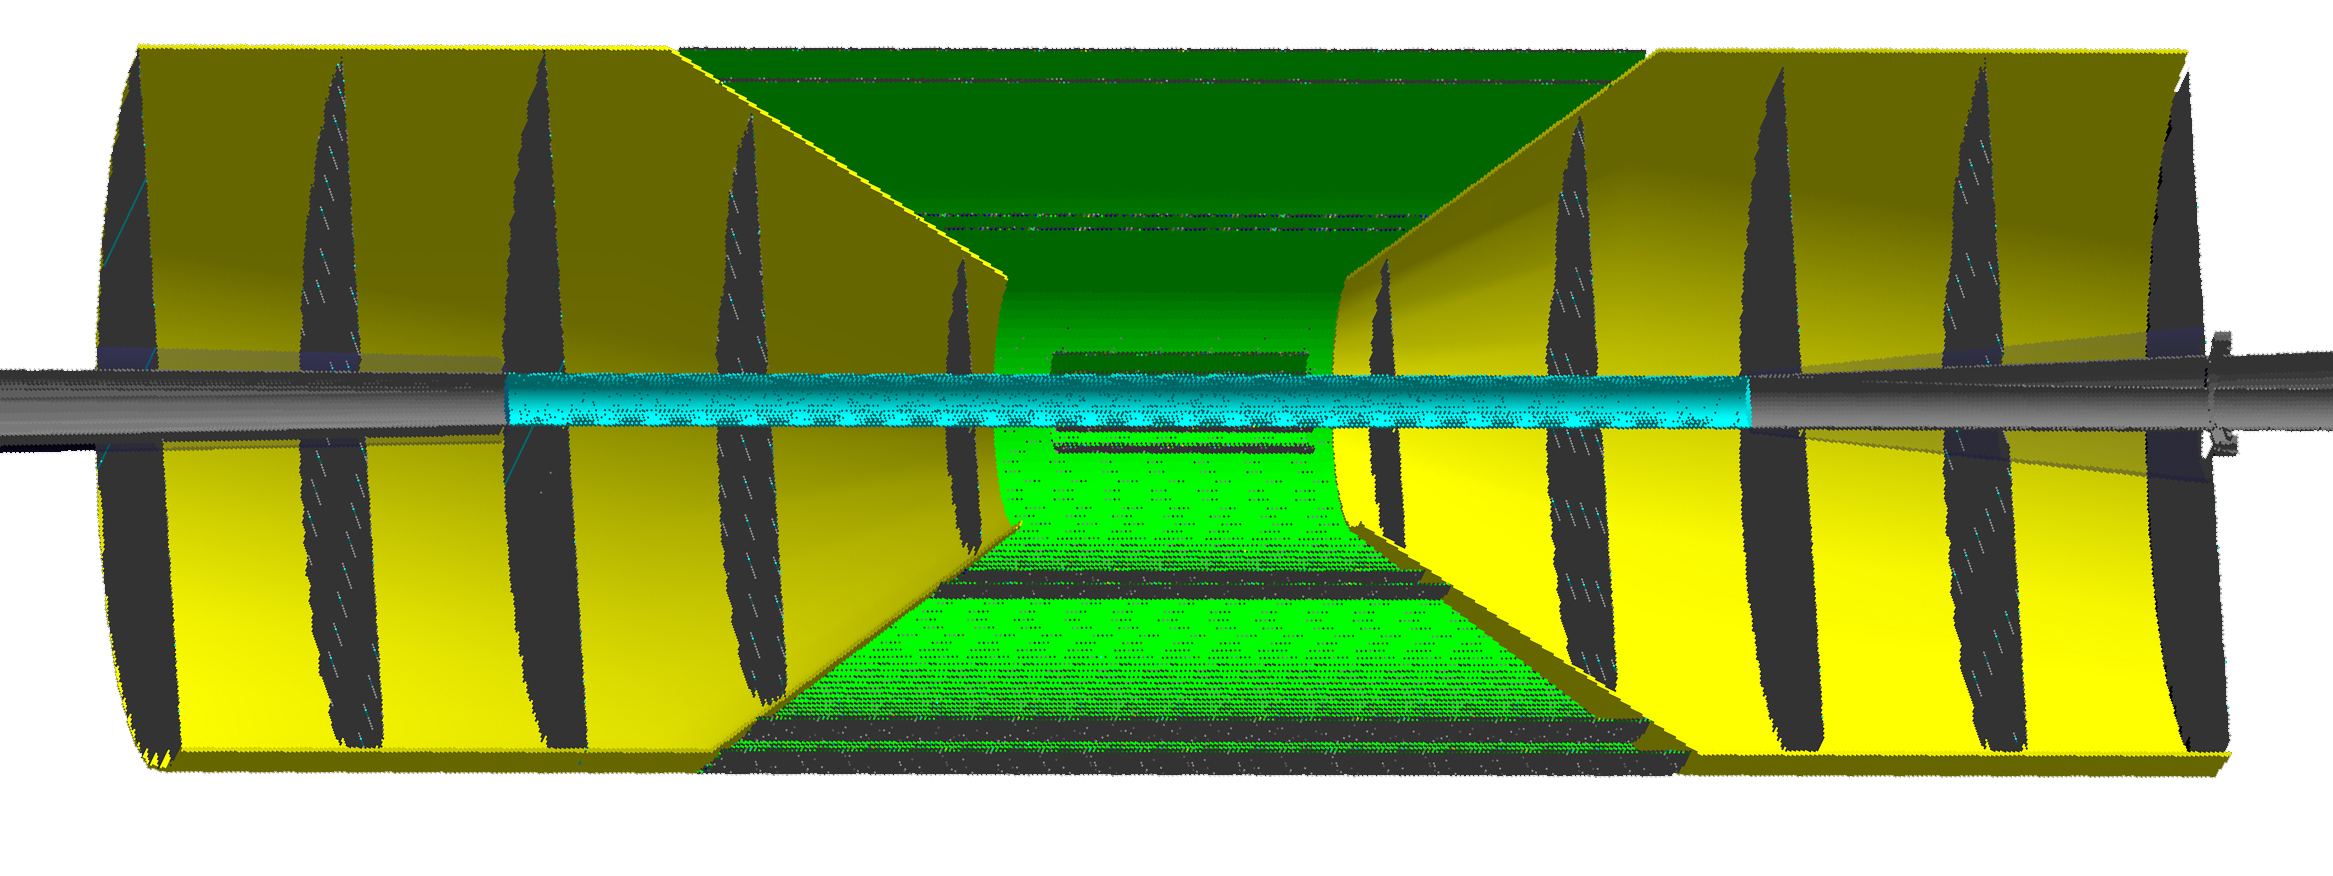
\includegraphics[width=0.495\textwidth]{EIC_Jets/all_si_model.jpg}
  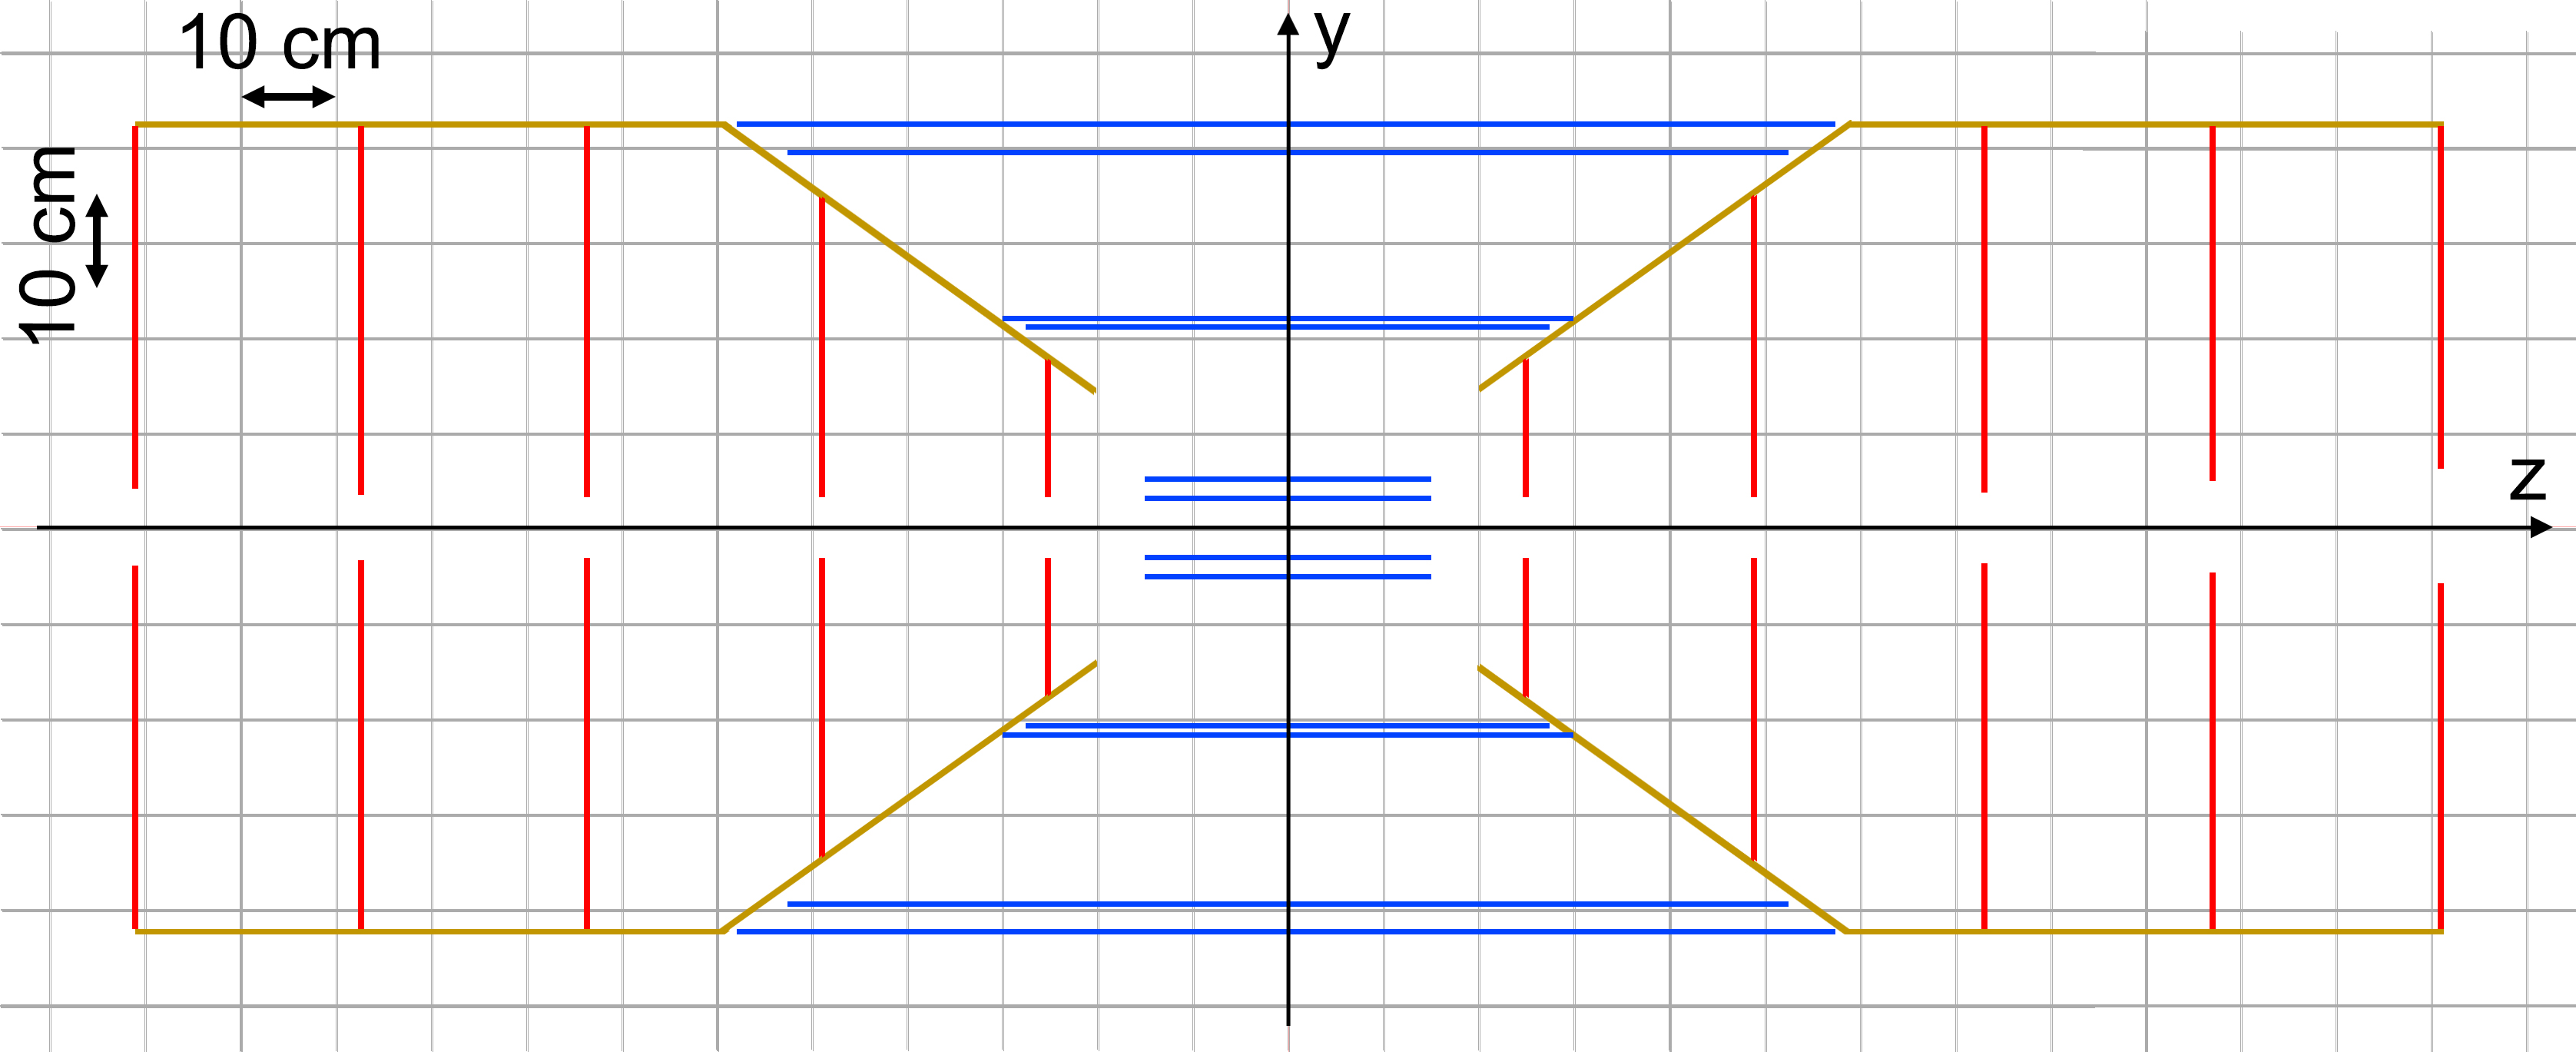
\includegraphics[width=0.495\textwidth]{EIC_Jets/diagram_allsi.jpg}
  \caption{All-silicon tracker geometry.
    Left: GEANT4 schematic of the tracker cross section. The barrel, disks, and support structure correspond to the green, dark-gray, and yellow components, respectively. The beryllium section of the beam pipe is shown in cyan. The rest of the beam pipe, which takes into account the expected electron-hadron-beam crossing angle is shown in light-gray.
  Right: detector schematic (side view). The barrel layers, disks, and support structure are represented in blue, red, and yellow, respectively. See text for details. Taken from \cite{Arrington2021}.}
  \label{fig:all_si_schematic}
\end{figure}

A schematic of the all-silicon tracker concept considered in this work is shown in Fig.~\ref{fig:all_si_schematic}.
The detector, designed within a generic EIC-detector R\&D effort~\cite{eRD16},
corresponds to a cylindrical tracker with radius of 43.2 cm and length of 242 cm along the $z$ direction and wrapped around the beam pipe and centered at the nominal IP (which corresponds to $(x,y,z)=(0,0,0)$). In the region $-79.8 < z < 66.8$ cm, the current design of the beam pipe corresponds to a beryllium cylinder of radius of 3.17 cm and a thickness of 760~\textmu m. Outside of this region, the beam pipe fans out to accommodate a beam-crossing angle of $\approx$25mrad. Inside the beam pipe, a vacuum is simulated. The rest of the geometry is embedded in an air volume.

The tracker coverage for low values of pseudorapidity, $\eta\equiv-{\mathrm ln}\big(\tan(\theta/2)\big)$ is provided by a barrel with 6 layers. The radii at which these layers are located and their corresponding lengths along $z$ are summarized on Table~\ref{tab:all_si:barrel} and illustrated in Fig.~\ref{fig:all_si_schematic} (right). They are laid out as three double layers to provide redundancy, and the middle double layer is placed equidistant between the inner and outer double layers to measure hits in the vicinity of the sagitta (vertical line from the midpoint of the chord to the arc itself, where the arc is simply the charged particles bend in the magnetic field) to optimize the momentum resolution. The pairing of the barrel layers also has the benefit of reducing the number of unique stave designs required.

The vertexing capabilities of the detector are driven primarily by the
first two layers. The innermost layer is placed as close to the beam pipe as possible, and the position of the second layer was varied until the optimal vertexing performance was found. Coverage at larger absolute values of pseudorapidity is provided by 5 disks in each direction. These disks are assembled by adding rectangular staves in parallel and giving each a length that fits within a circle of radius $R$, the disk outer radii presented in Table~\ref{tab:all_si:disks}, along with their $z$ positions and inner radii; see Fig.~\ref{fig:all_si_schematic} (right).

Given the rectangular geometry of the staves, the hole through which the beam pipe passes is shaped as a square with sides equal to twice the inner radii presented in Table~\ref{tab:all_si:disks}.
While the disks on either side of the $x-y$ plane are positioned at the same distance from the center of the detector and their outer radii are the same, their inner radii are optimized to be as close to the beam pipe as possible. Thus, the acceptance limit at high $|\eta|$ is given by the beam-pipe geometry.
Given the asymmetric nature of the EIC collisions ($i.e.$ electrons colliding with protons or nuclei with different lab-frame energies), a potential future improvement is to optimize the disk layout separately for the forward and backward regions.
An odd number of disks is favored to measure hits in the vicinity of the sagitta, thus achieving a better resolution.
The transition between the barrel and the disks occurs at
$|\eta|\approx 1.1$.

\begin{figure}[htbp]
    \centering
    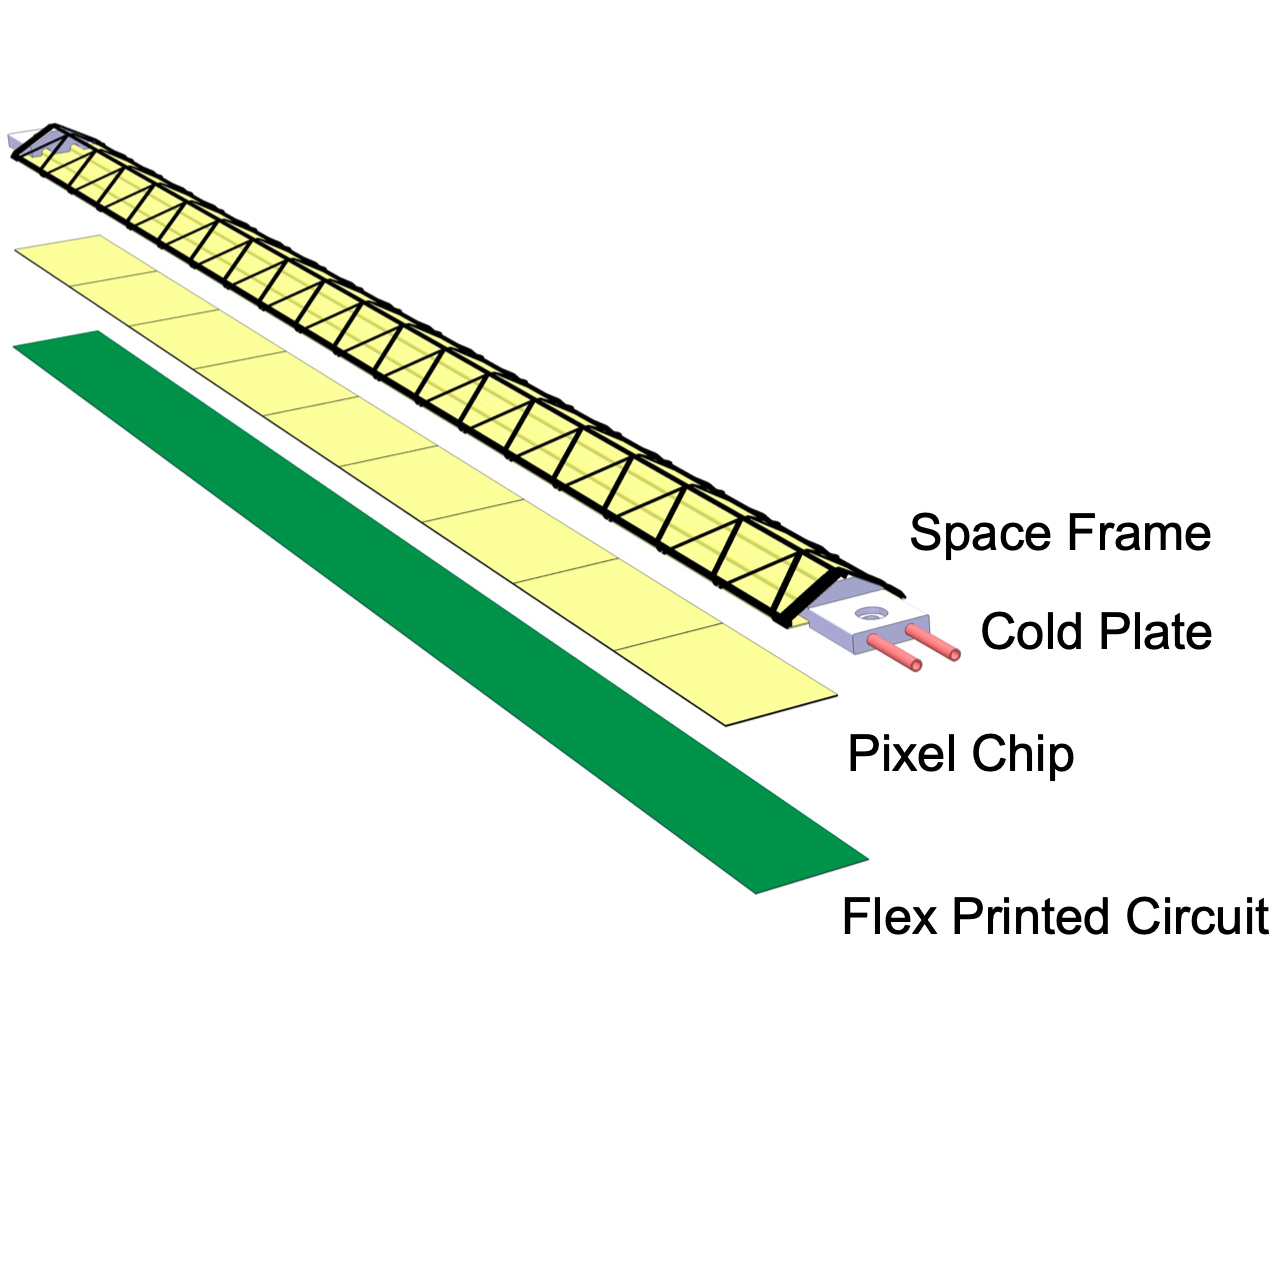
\includegraphics[width=0.40\textwidth]{EIC_Jets/alice_its2_stave.jpg}
    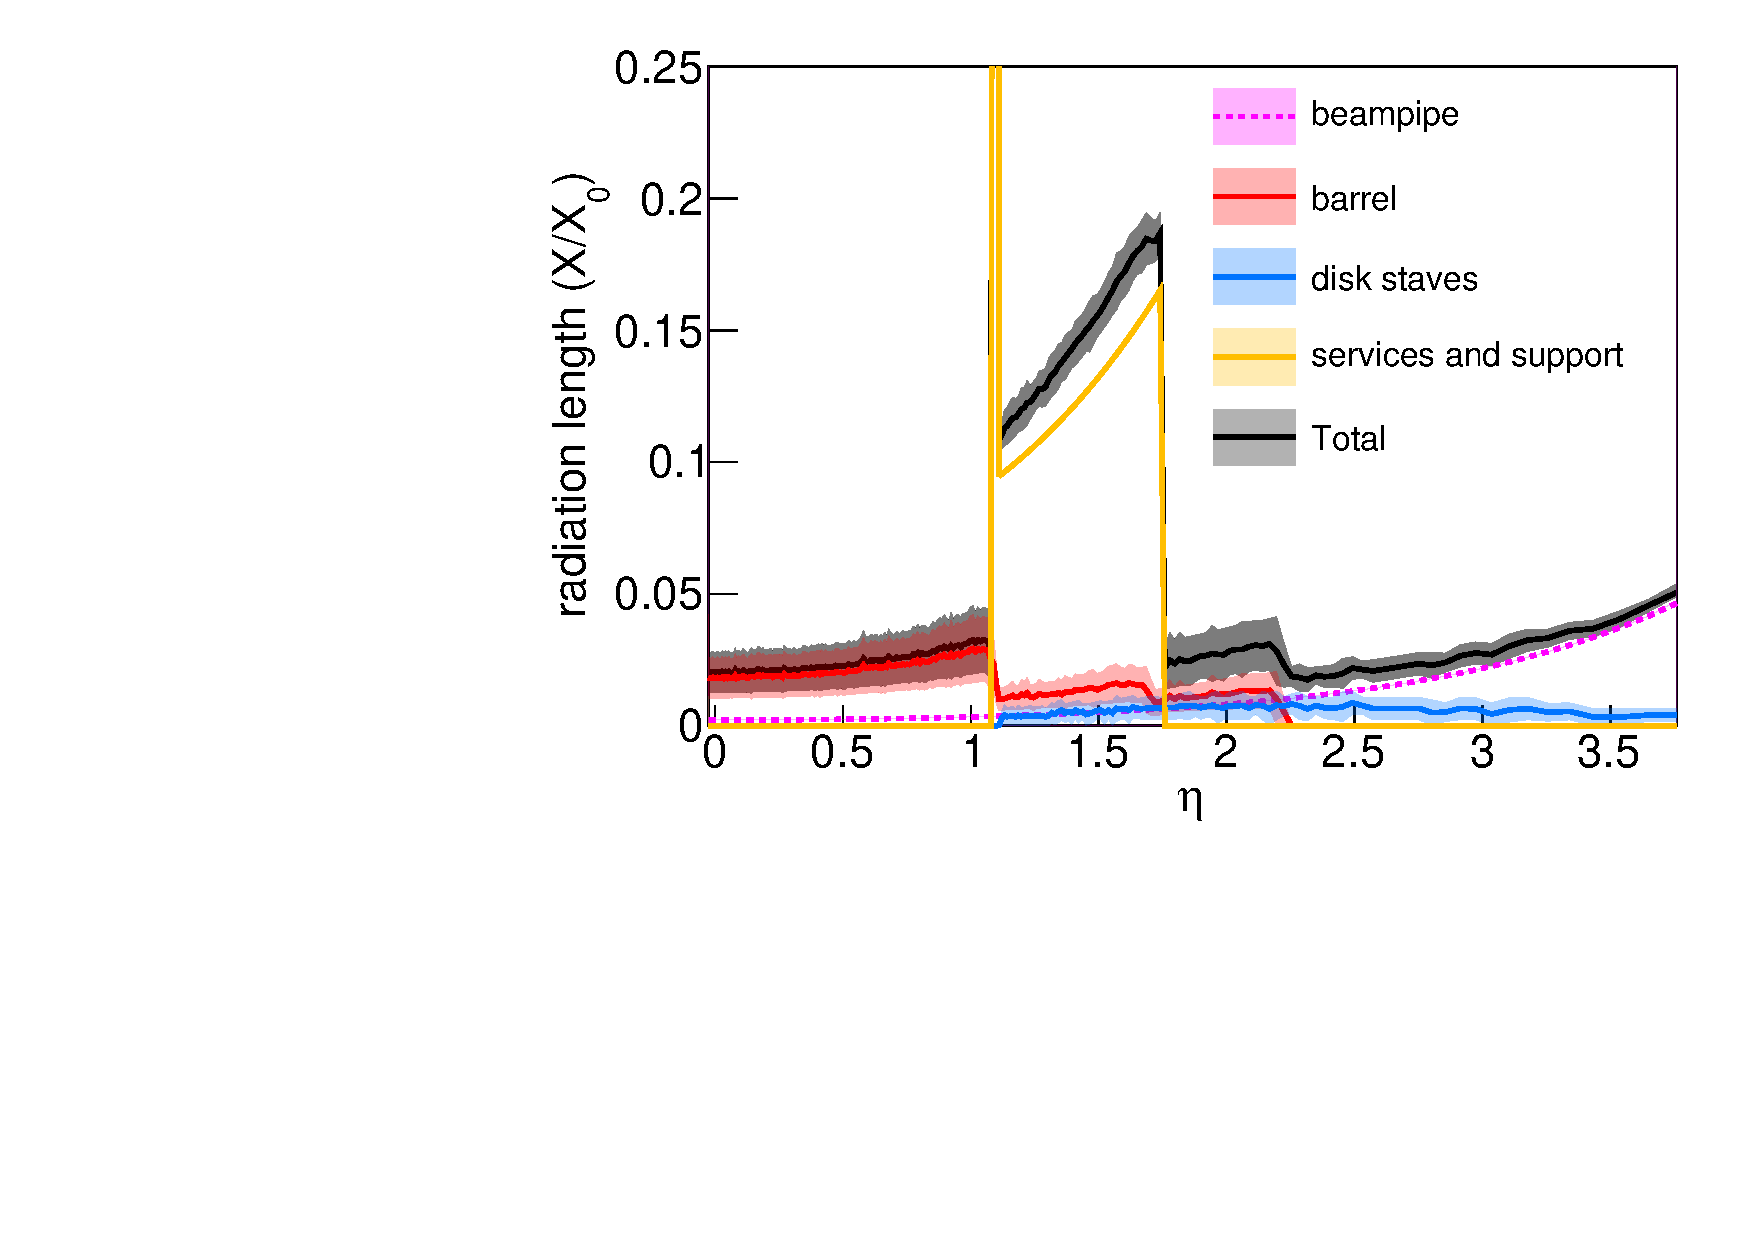
\includegraphics[width=0.59\textwidth]{EIC_Jets/mat_scan.pdf}
    \caption{Detector material budget.
    Left: schematic of the ALICE ITS2 inner-barrel staves used in the all-silicon tracker design presented here. Schematic taken from Fig.1.3 in~\cite{Abelevetal:2014dna}.
    Right: all-silicon tracker material scan.
    The dashed magenta line corresponds to the material from the beam pipe.
    The barrel and disk contributions are shown in red and blue, respectively.
    The aluminum support structure is shown in yellow.
    The total contribution is shown in black.
    See text for details.
    }
    \label{fig:material}
\end{figure}

\begin{table}
  \centering
\caption{Barrel-layer radii and lengths.}
\label{tab:all_si:barrel}
\resizebox{0.5\textwidth}{!}{\begin{tabular}{c|ccc}
~~Barrel~~  & ~~radius~~    & ~~length along z~~        \\
layer   & {[}cm{]}  & {[}cm{]}              \\
  \hline \hline
1       & 3.30      & 30                    \\
2       & 5.70      & 30                    \\
\hline
3       & 21.00     & 54                    \\
4       & 22.68     & 60                    \\
\hline
5       & 39.30     & 105                   \\
6       & 43.23     & 114                    
\end{tabular}}

\caption{Disk $z$ position and inner and outer radii.}
\label{tab:all_si:disks}
\resizebox{0.7\textwidth}{!}{\begin{tabular}{c|ccc}
Disk  		& ~~z position~~	& outer 			& inner 			\\
~~number		& {[}cm{]}      & ~~radius {[}cm{]}~~	& ~~radius {[}cm{]}~~	\\
\hline \hline
-5			& -121		    & 43.23			    & 4.41			    \\
-4			& -97		    & 43.23			    & 3.70			    \\
-3			& -73		    & 43.23			    & 3.18			    \\
-2			& -49		    & 36.26			    & 3.18			    \\
-1			& -25		    & 18.50			    & 3.18			    \\
\hline
1           & 25            & 18.50			    & 3.18 			    \\
2           & 49            & 36.26			    & 3.18 			    \\
3           & 73            & 43.23			    & 3.50 			    \\
4           & 97            & 43.23			    & 4.70 			    \\
5           & 121           & 43.23             & 5.91
\end{tabular}}
\end{table}


Both the barrel layers and the disks are made up of realistic staves modeled after the ALICE-ITS2-upgrade inner-barrel staves~\cite{Abelevetal:2014dna,Keil:2015vta,Reidt:2016ysg}
and shown in Fig.~\ref{fig:material} (left).
Besides the active silicon volume, each stave includes components such as carbon-fiber support structures and water cooling pipes, which combined correspond to an average material budget of 0.3$\%~X_0$ per stave.
The total amount of material that these staves contribute to the all-silicon tracker geometry is shown in Fig.~\ref{fig:material} (right)
Since the staves create a periodic but $\phi$-varying structure (where $\phi$ corresponds to the azimuth), the geometry is scanned around the azimuth for a fixed $\eta$, and the minimum and maximum amounts of material found define the boundaries of the uncertainty band.
With the current configuration, the material budget contributed by the barrel and disk staves is $<5\%X~0$.

The attributes of the sensor used in the simulations are taken from the eRD25 and EIC Silicon Consortium~\cite{eRD25} descriptions of the projected properties of an EIC specific Monolithic Active Pixel Sensor (MAPS) currently under development.
The sensor silicon pixels have a pitch of 10$\times$10\textmu m$^2$ (corresponding to a point resolution of 10/$\sqrt{12}$ \textmu m) and silicon thickness of 50 \textmu m. While this simulation effort uses 0.3$\%~X_0$ for the inner two tracking layers, there are ongoing R\&D efforts to use stitched, thinned and bent air-cooled silicon to allow the vertexing layers to become as thin as 0.05$\%~X_0$~\cite{its3det}. 

As part of the EIC Yellow Report effort, projections were generated for both the radiation length of staves and discs~\cite{leo} based on the eRD25 EIC specific sensor and for the services (location and composition) and mechanical supports~\cite{leo2} that would be required to complete a tracking detector. These projections, which were only available after most of the work presented here, are referenced for completeness and are reasonably consistent with what is used in the shown simulation for material in the tracking detectors acceptance.

The detector is complemented with a simplistic conical aluminum support structure with a thickness of 5mm which is tapered for $z>58$ cm. As shown in Fig.~\ref{fig:material} (right), this support structure adds a significant amount of material 
to the detector. However, the projective design concentrates this material into a narrow pseudorapidity range at $|\eta|=1.1$.
More realistic support structures (likely made of carbon-fiber composite) and services are still to be implemented.  
An earlier notional all-silicon detector extended out to a radius of 75 cm \cite{Klein:2020sts}; a larger detector can offer improved momentum resolution, at a cost in larger silicon area, and hence cost.  This study also considered the possibility of using timing to improve resolution for low-momentum particles, but this is difficult with the smaller 43 cm lever arm.

% \section{All-Silicon Tracker Performance}
% \label{sec:performance}

% This geometry was implemented in GEANT4 and
% studied within the full Monte-Carlo framework for detector simulation, Fun4All~\cite{Fun4All,Pinkenburg:2011zza,Pinkenburg:2005zza}.
% Performance studies were carried out by generating charged particles ($e.g.$ pions, electrons, protons, and muons) from the nominal IP in the momentum range $0 < p < 30$ GeV$/c$ and over the entire detector acceptance ($i.e.$ $|\eta|<4$ and $0<\phi<2\pi$).
% The two magnetic fields considered for the simulations correspond to solenoidal field maps for the BeAST~\cite{Beast1,Beast2} and BaBar~\cite{Babar} magnets, with peak intensities of 3.0~T and 1.4~T, respectively.
% The hits resulting from the interaction between the generated particles and the detector (which was setup with a hit efficiency at 100\%) were combined into tracks, and differences between the variables generated and reconstructed in the simulation (labeled `truth' and `reco', respectively) were used to characterize various detector resolutions. 
% Pattern recognition for combining hits
% into reconstructed tracks 
% is seeded
% using truth-track information. Thus, final efficiency studies are not feasible at the moment and will be carried out when more realistic seeding algorithms are implemented.

% % \begin{figure}[htbp]
% %     \centering
% %     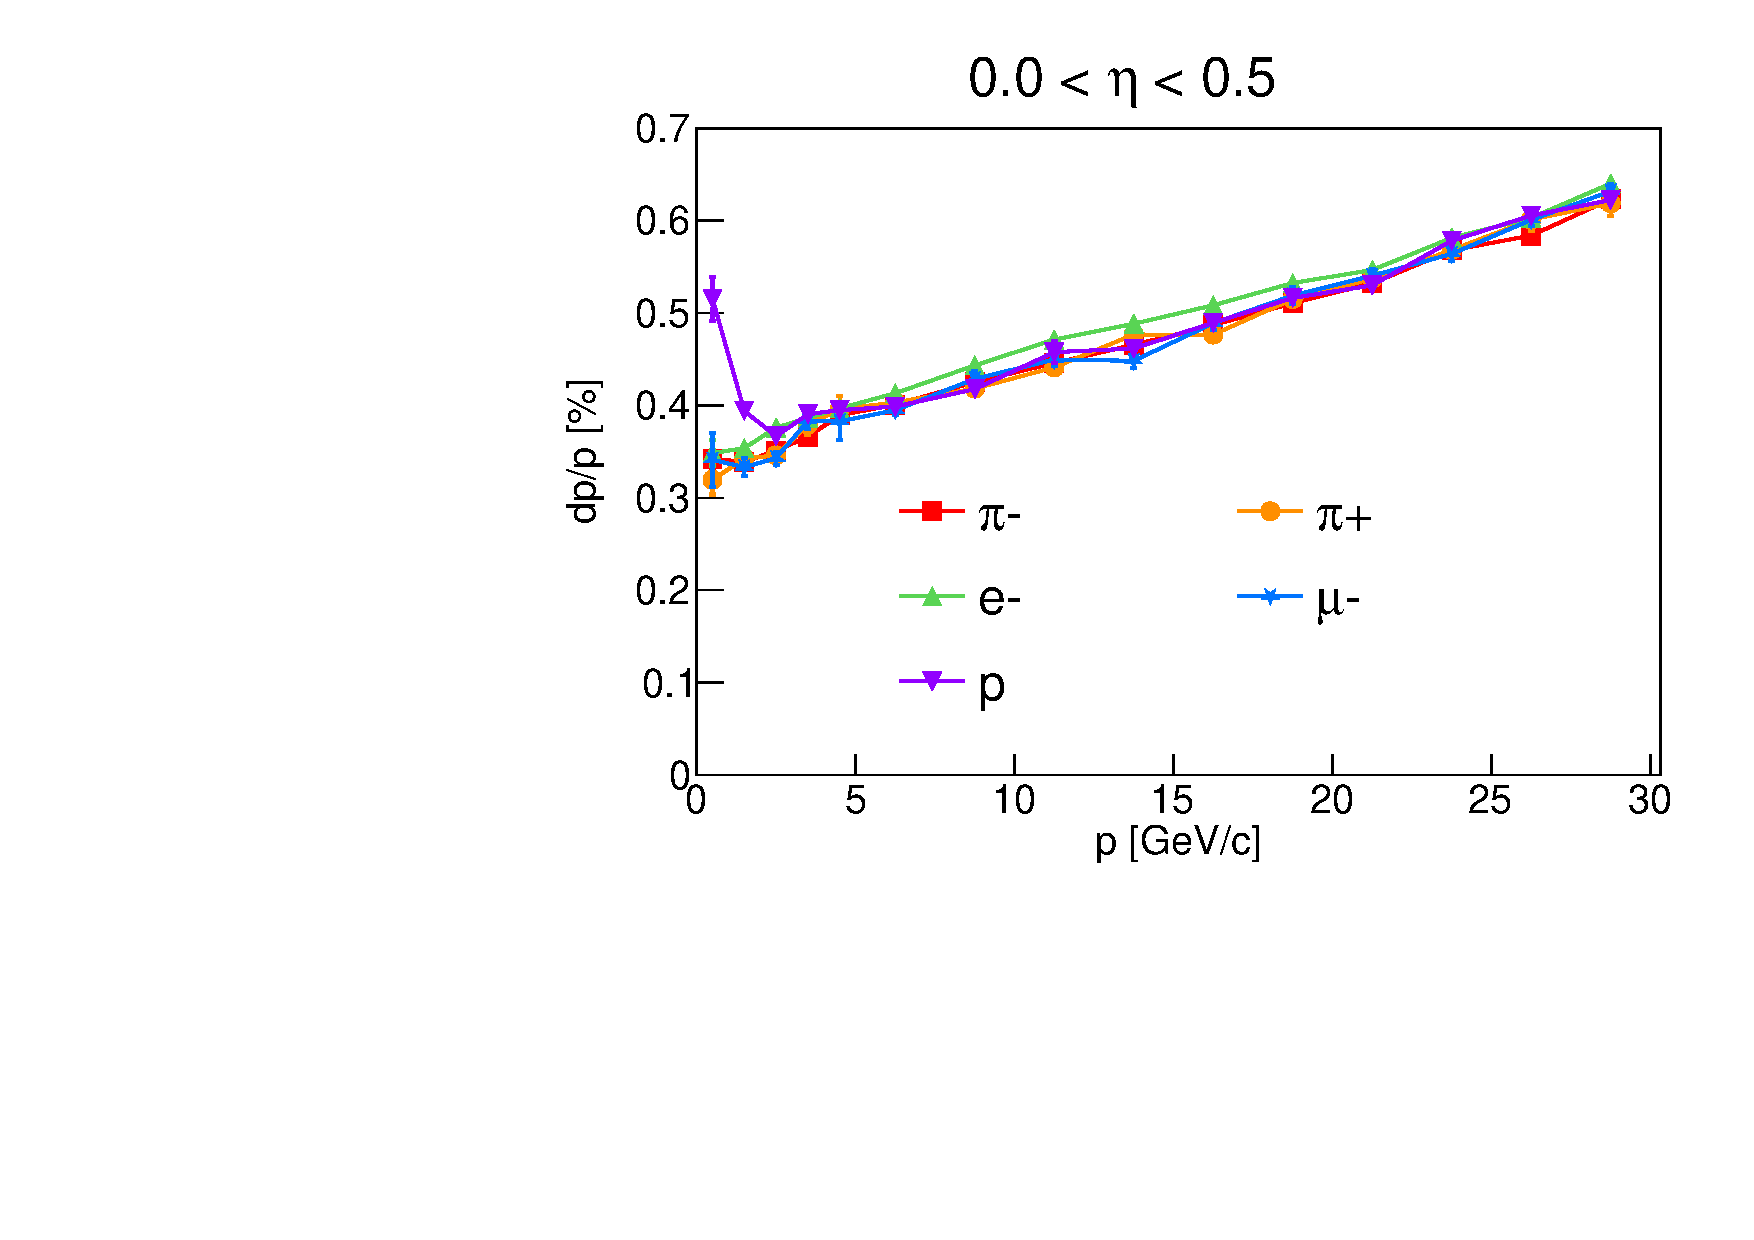
\includegraphics[width=0.45\textwidth]{EIC_Jets/results_particle_comp_c2.pdf}
% %     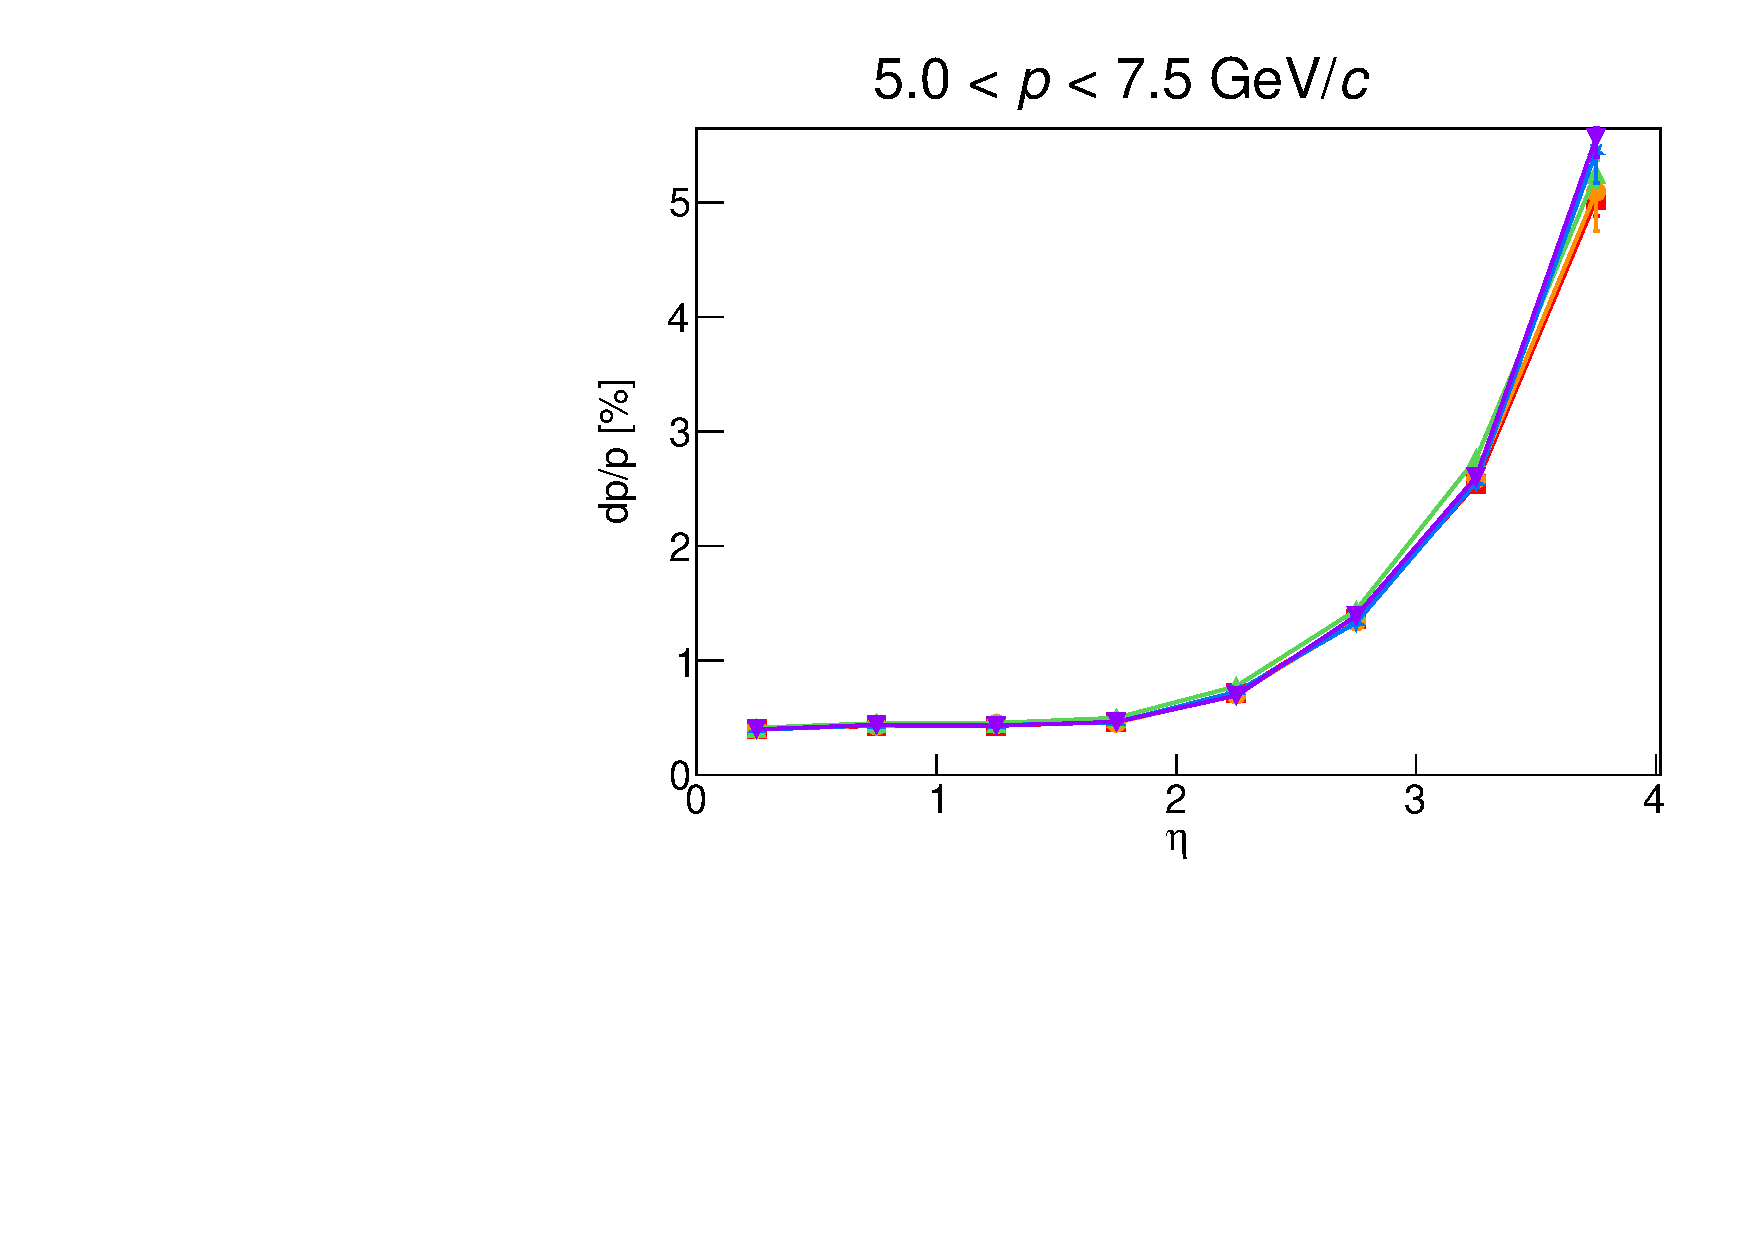
\includegraphics[width=0.45\textwidth]{EIC_Jets/results_particle_comp_c3.pdf}
% %     \caption{
% %     Momentum resolution for different particles in the 3.0~T magnetic field.
% %     Left: $dp/p$ as a function of momentum in the $0 < \eta < 0.5$ range.
% %     Right: $dp/p$ as a function of pseudorapidity in the $5.0 < p < 7.5$GeV/$c$ range.
% %     See text for details.}
% %     \label{fig:diff_particles}
% % \end{figure}

% \begin{figure}[htbp]
%     \centering
%     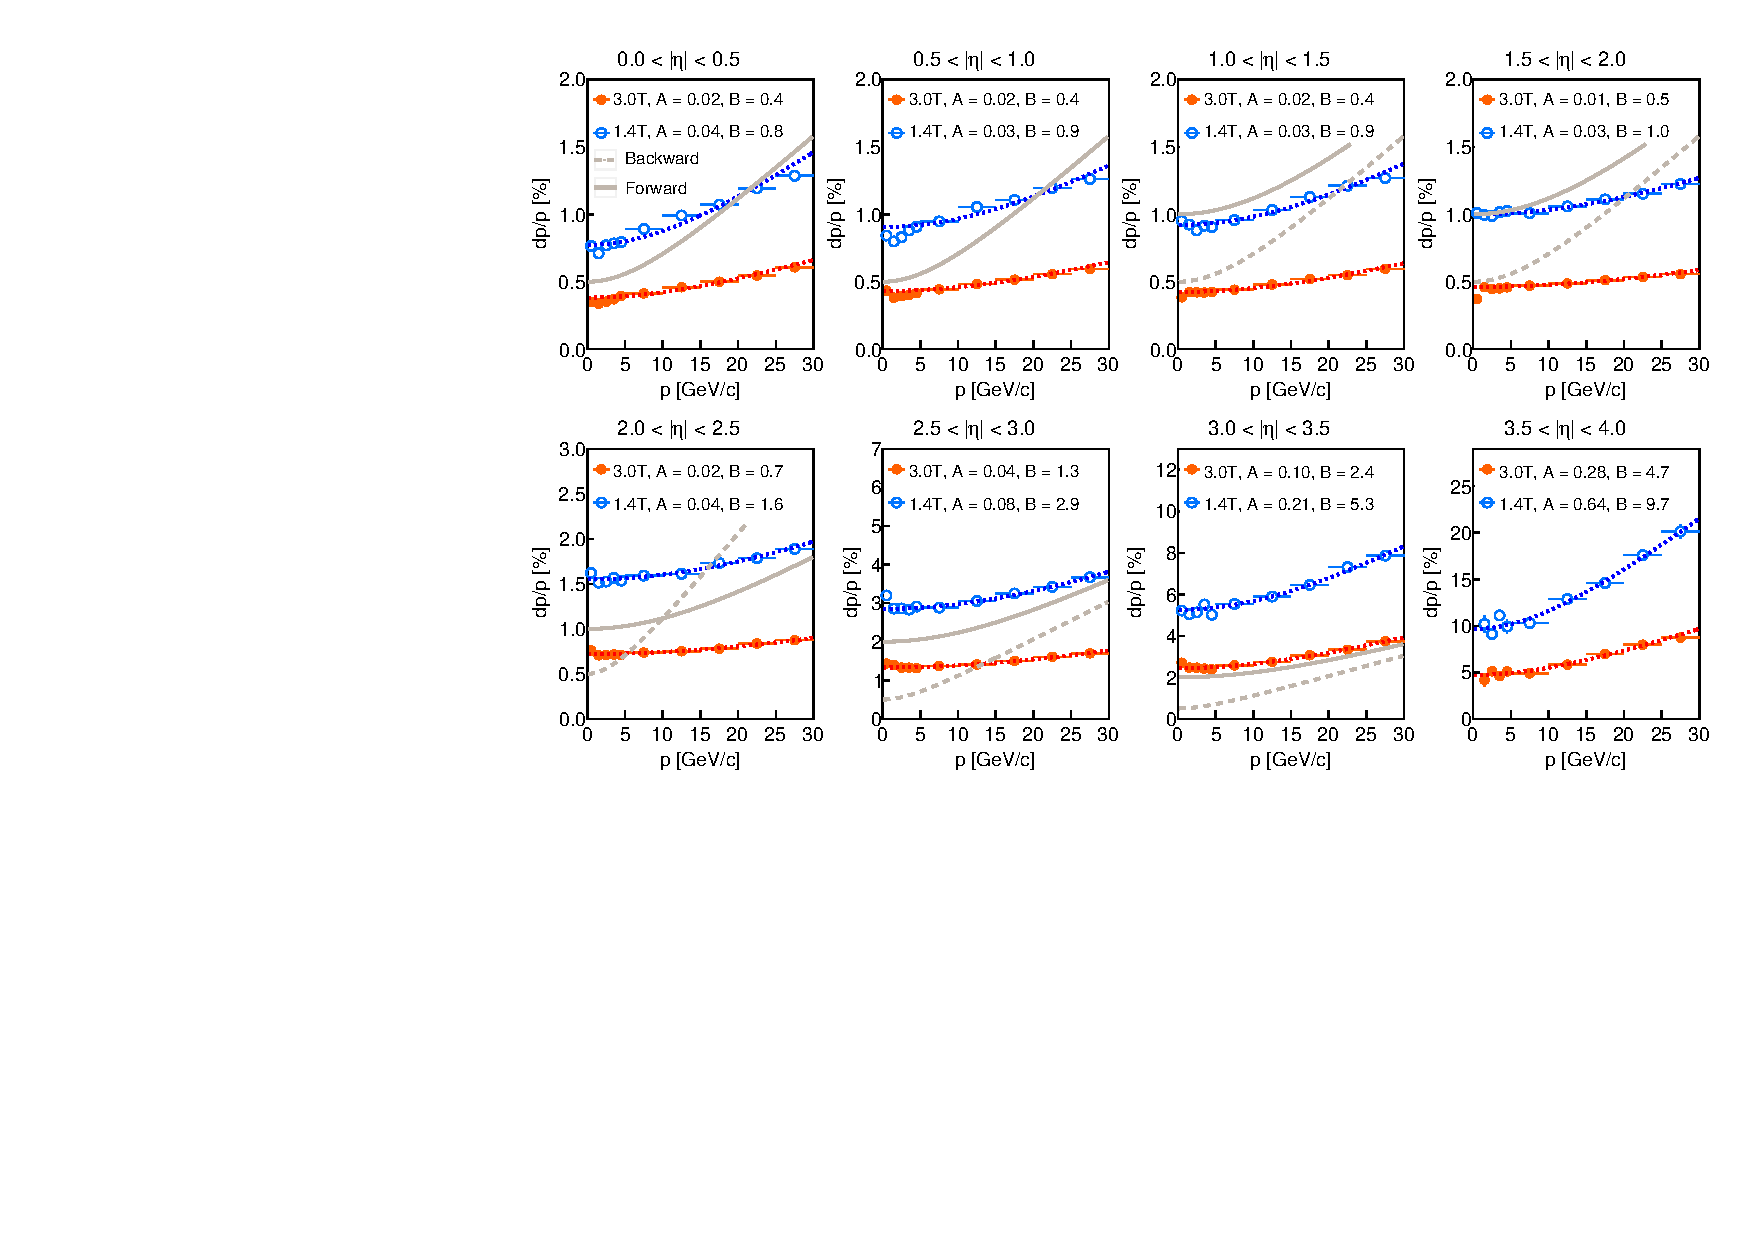
\includegraphics[width=0.95\textwidth]{EIC_Jets/results_mom_res_fits.pdf}
%     \caption{Momentum resolution as a function of momentum for several
%     pseudorapidity bins. The markers correspond to the resolutions extracted
%     from the simulations, and the lines correspond to fits to such resolution curves.
%     The orange (filled) and blue (open) circles correspond to simulations carried out with the BeAST (3.0~T) and BaBar (1.4~T) field maps respectively.
%     The functional form used in the fits is $dp/p=Ap\oplus B$, and the parameters $A \ [\%/({\mathrm GeV}/c)]$ and $B \ [\%]$ are given in the plots. The EIC physics requirements~\cite{DMtable:2020} are shown as gray lines for $|\eta|<3.5$. In the cases where the forward and backward requirements are different, the backward requirements are shown as dashed lines.}
%     \label{fig:all_si:mom_res_param}
% \end{figure}

% \begin{figure}[htbp]
%     \centering
%     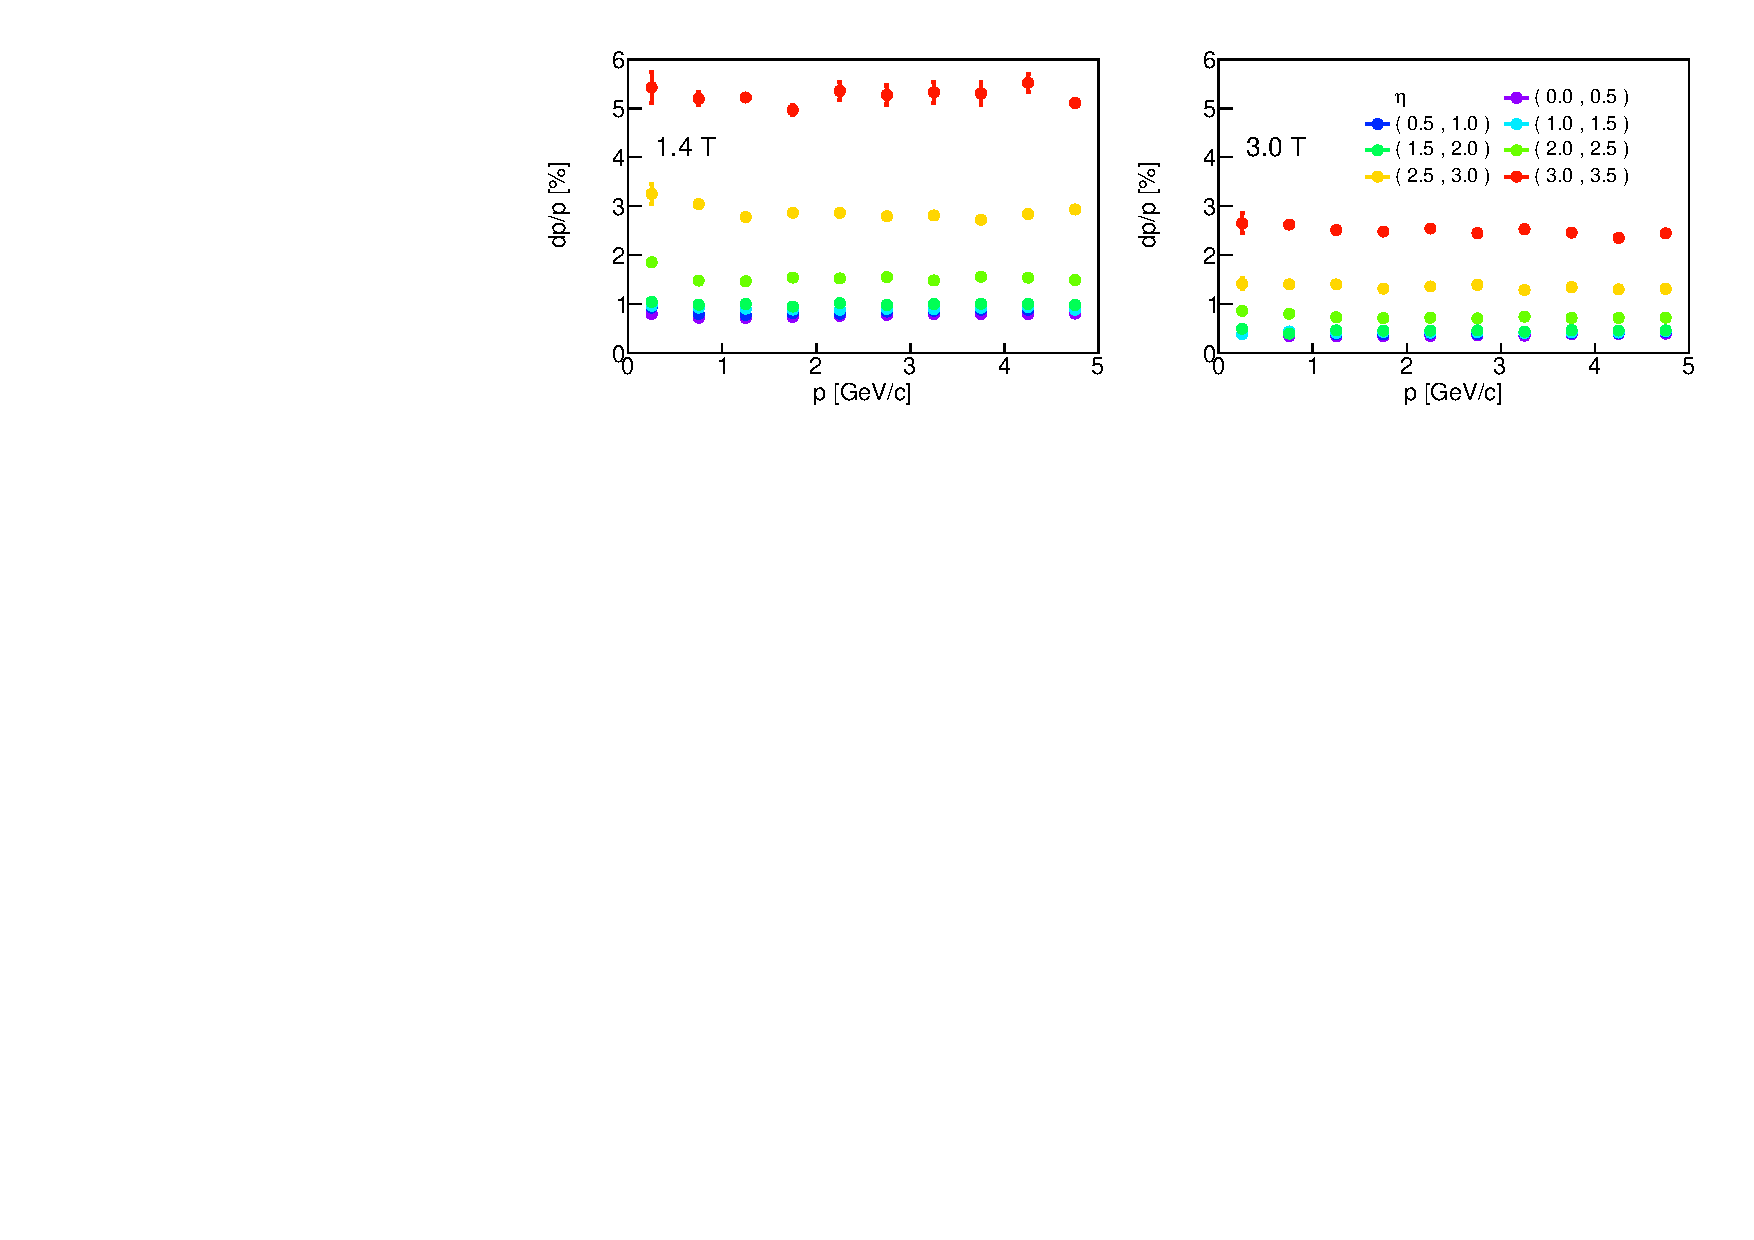
\includegraphics[width=0.95\textwidth, clip]{EIC_Jets/mom_res_lowp.pdf}
%     \caption{Momentum resolution as a function of momentum for several
%     pseudorapidity bins in the low-momentum region. Left: 1.4~T magnetic field. Right: 3.0~T magnetic field.}
%     \label{fig:all_si:mom_res_lowp}
% \end{figure}

% The momentum resolution, $dp/p$, is defined as the standard deviation of the $(|\vec{p}_{\mathrm truth}|-|\vec{p}_{\mathrm reco}|)/|\vec{p}_{\mathrm truth}|$ distribution, where $|\vec p|$ is the absolute value of the particle momentum.

% Detailed momentum-resolution studies for pions are shown for both magnetic-field settings in Fig.~\ref{fig:all_si:mom_res_param} \cite[Arrington2021]. The performance of various particles was studied and found to be extremely similar down to very low \pt. As a results, detailed studies will be shown only for pions.
% As expected from the leading-order $\sim1/B$ dependence of the momentum resolution, doubling the magnetic-field intensity improves the momentum resolution by a factor of $\approx 2$. Momentum resolutions are typically parametrized by the function $dp/p = A \cdot p \oplus B$, where $A$ and $B$ are fit parameters and $\oplus$ indicates sum in quadrature. The resulting fits and the fit parameters are shown in the figure.
% Also shown as gray lines are the requirements determined by the physics working groups in the EIC Yellow Report effort~\cite{DMtable:2020}. 
% In the case of the 3.0T field, the initial tracker design satisfies the physics requirements over the entire $0 < p < 30$GeV$/c$ range for $-2.0 < \eta < 3.0$ but falls short, especially for lower-momentum particles, outside of this range.
% At 1.4T, there is no pseudorapidity range where the tracker can satisfy the requirements over the entire momentum range.
% While the momentum resolutions are better with the 3.0T magnet, the 1.4T magnet has advantages: such a magnet already exists (reducing the cost of the detector) and the smaller field intensity allows lower-transverse-momentum particles to be measured.
% Momentum resolutions for particles with $p<5{\mathrm GeV}/c$ are shown in Fig.~\ref{fig:all_si:mom_res_lowp}.

% % \subsection{Further momentum resolution optimization}
% % \label{sec:optimization}

% % To study whether the momentum resolution could be improved at forward and backward pseudorapidities, where there is tension between the tracker performance and physics requirements, the detector was complemented with additional tracking stations taking into consideration the space currently projected to be available according to the Central Detector/Integration \& Magnet Working Group~\cite{ayk}. Placing such complementary trackers away from the interaction point increases the field integral, $\int B\cdot\mathrm{d}l$, thus improving the momentum resolution, and no specific detectors are planned to be installed between the backward station and the all-silicon tracker. We examined the impact of adding methane-based gas electron multiplier (GEM) detectors or additional silicon disks in the backward and forward regions at $z = -180$ and 300cm, respectively.
% % The resulting momentum resolutions in the backward region are shown in Fig.~\ref{fig:gem_back}.
% % Complementing the all-silicon tracker with a 50\textmu${\mathrm m}$-resolution GEM station yields a small improvement, mainly for low-momentum particles, while a 10\textmu${\mathrm m}$-pixel silicon disk significantly improves the momentum resolution in the far-backward region (negative $\eta$), by a factor of two or more for high-momentum particles.

% % \begin{figure}[htbp]
% %     \centering
% %     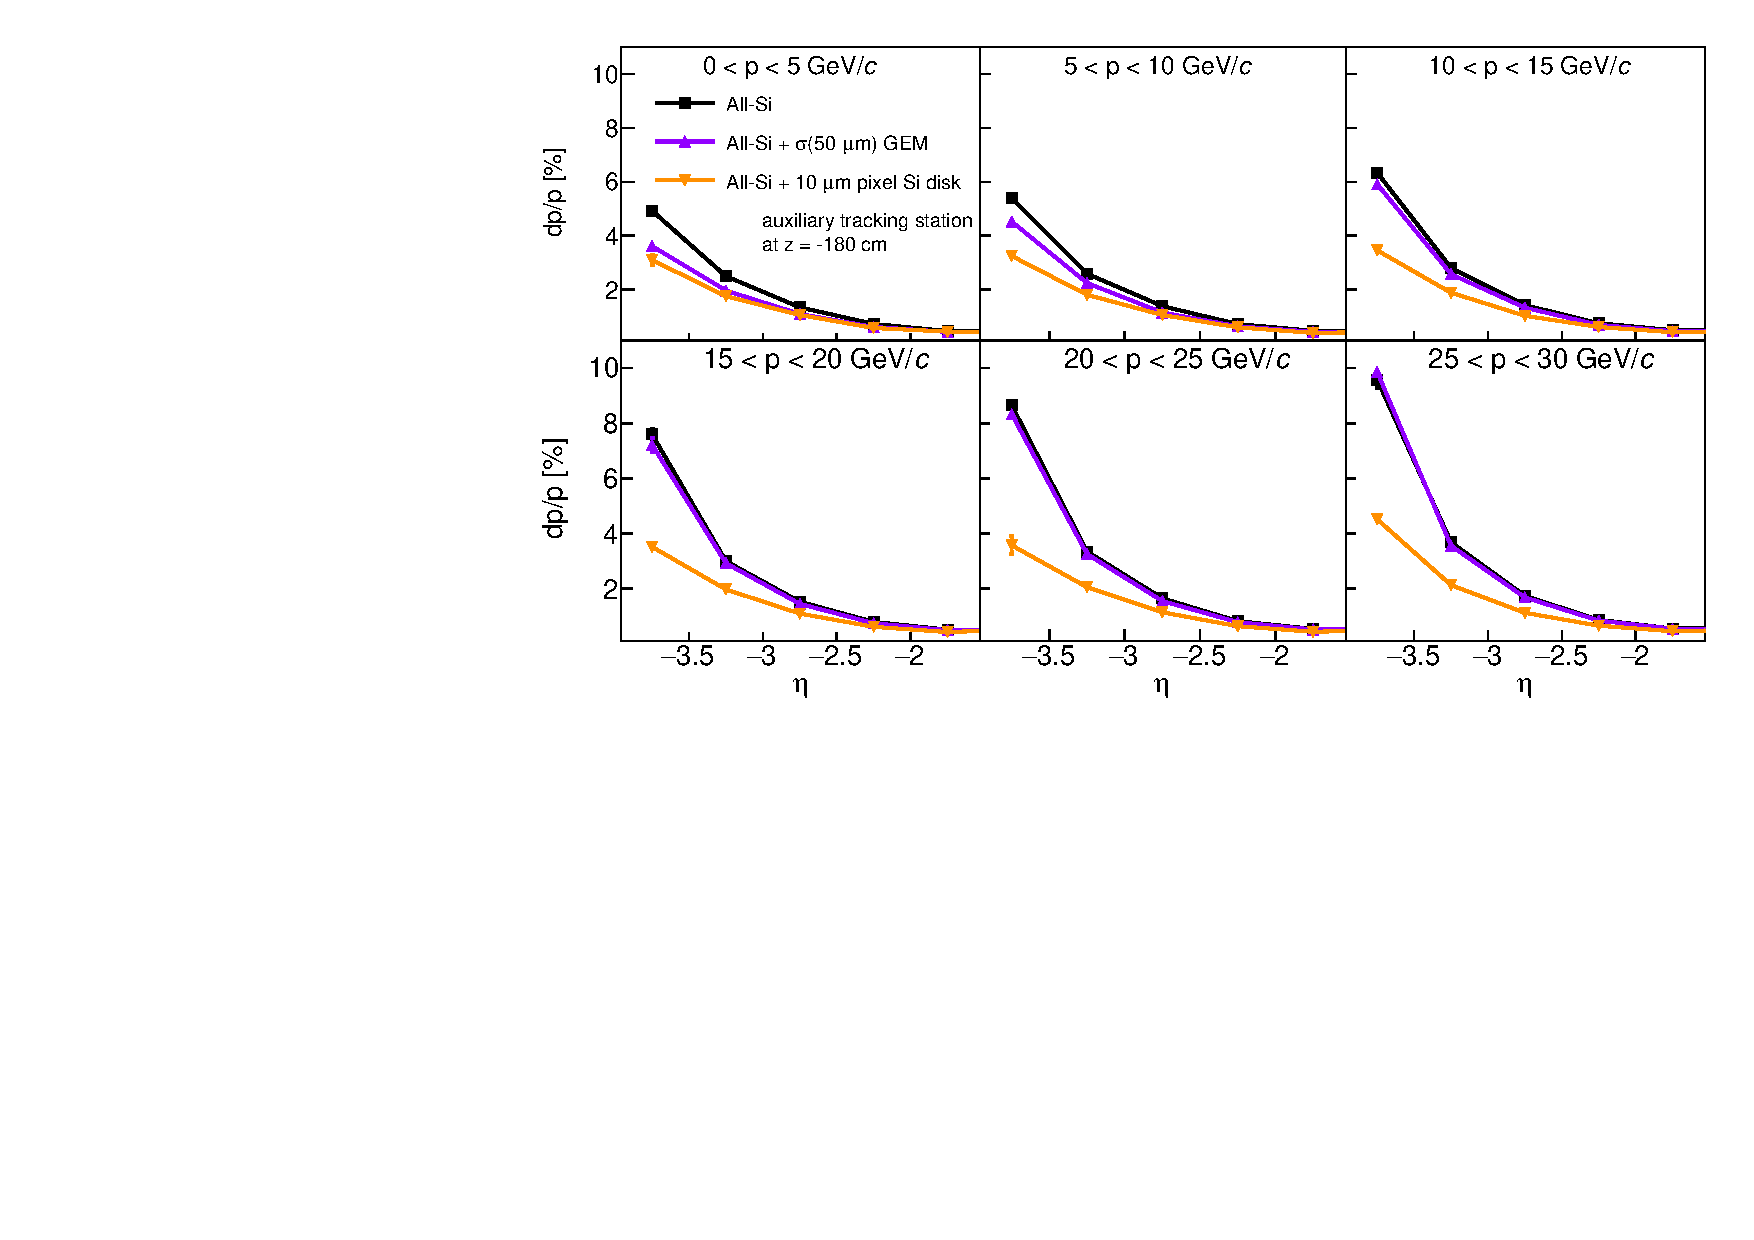
\includegraphics[page=1,width=0.85\textwidth]{EIC_Jets/all_si_GEM_si_disk.pdf}
% %     \caption{Momentum resolution as a function of pseudorapidity in the backward region. The all-silicon tracker standalone performance is shown in black squares. The purple triangles and orange inverted triangles describe the momentum resolution achieved by complementing the all-silicon tracker with a 50\textmu${\mathrm m}$-resolution GEM station or a 10\textmu${\mathrm m}$-pixel silicon disk at $z=-180$cm, respectively. In this region, the all-silicon tracker complemented with a silicon disk offers a significantly better performance. See text for details.}
% %     \label{fig:gem_back}
% % \end{figure}

% % \begin{figure}[htbp]
% %     \centering
% %     \includegraphics[page=2,width=0.85\textwidth]{EIC_Jets/all_si_GEM_si_disk.pdf}
% %     \caption{Momentum resolution as a function of pseudorapidity in the forward region. The all-silicon tracker standalone performance is shown in black squares. The purple triangles and orange inverted triangles describe the momentum resolution achieved by complementing the all-silicon tracker with a 50\textmu${\mathrm m}$-resolution GEM station or a 10\textmu${\mathrm m}$-pixel silicon disk at $z=300$cm, respectively.
% %     In this region, a RICH detector is placed in the space between the all-silicon tracker and the complementary tracking station.
% %     The all-silicon tracker complemented with a GEM offers a performance comparable to that of the tracker complemented with a silicon disk (except in the highest momentum bin shown). See text for details.}
% %     \label{fig:gem_forw}
% % \end{figure}

% % In the forward region, the complementary station is placed behind a Ring Imaging Cherenkov (RICH) detector. The RICH material budget was provided by the PID detector working group~\cite{cisbani} and it corresponds to a dual-radiator (aerogel and C$_2$F$_6$) device.
% % The resulting momentum resolutions are shown in Fig.~\ref{fig:gem_forw}.
% % In this region, a 50\textmu${\mathrm m}$-resolution GEM provides a momentum-resolution enhancement comparable to that of a 10\textmu${\mathrm m}$-pixel silicon disk except in the highest momentum bin. Both provide a small improvement in the resolution in the far-forward region for momenta above 5 GeV/$c$.
% % In practice, the magnetic-field lines are expected to be shaped in such a way that bending inside the $\sim150$-cm-long RICH will be minimal, and the momentum-resolution improvement will be smaller in the forward region. More detailed magnetic-field simulations are needed to study this effect.
% % The complementary tracking stations were simulated with acceptance in the region $|\eta|>1.2$. Nevertheless, it can be seen in Figs.~\ref{fig:gem_back}~and~\ref{fig:gem_forw} that their impact is negligible for $|\eta|<2.5$. Thus, smaller tracking stations can be constructed to complement the tracker in the EIC.

% % \subsection{Pointing resolution}
% % \label{sec:pointing}

% % In addition to measuring the momenta of particles, the silicon tracker must be able to reconstruct secondary vertices and project track trajectories to the outer detector systems.
% % The Distance of Closest Approach (DCA) is defined as the spatial separation between the primary vertex and the reconstructed track projected back to the $z$ axis (DCA$_{z}$) or to the $x-y$ plane (DCA$_{r\phi}$). The DCA resolutions were determined as the standard deviation of
% % normal functions fitted to the DCA$_{z}$ and DCA$_{r\phi}$ distributions.
% % DCA-resolution results as a function of transverse momentum ($p_T$) for pions are shown in Figs.~\ref{fig:all_si:dca_z_res_param}~and~\ref{fig:all_si:dca_t_res_param}.
% % The resulting distributions were characterized via fits with the functional form $\sigma({\mathrm DCA})=A/p_T\oplus B$.
% % The fits and fit parameters are presented in the figures. It is clear that the DCA resolutions are insensitive to the magnetic field.

% % \begin{figure}[htbp]
% %     \centering
% %     \includegraphics[width=0.95\textwidth,page=3]{EIC_Jets/results_vtx_res_fits.pdf}
% %     \caption{Longitudinal DCA resolution vs. transverse momentum for several pseudorapidity bins.
% %     The circles correspond to the resolutions extracted from the simulations, and the lines correspond to fits to the resolution of the form $\sigma({\mathrm DCA}_z)=A/p_T\oplus B$,
% %     with the parameters
% %     $A \ [$\textmu${\mathrm m} \cdot {\mathrm GeV}/c]$ and $B \ [$\textmu${\mathrm m}]$ given in the figure. 
% %     The orange, filled and blue, open circles correspond to simulations using the BeAST (3.0~T) and BaBar (1.4~T) field maps.}
% %     \label{fig:all_si:dca_z_res_param}
% % \end{figure}

% % \begin{figure}[htbp]
% %     \centering
% %     \includegraphics[width=0.95\textwidth,page=4]{EIC_Jets/results_vtx_res_fits.pdf}
% %     \caption{Transverse DCA resolution vs. transverse momentum for several pseudorapidity bins.
% %      The circles correspond to the resolutions extracted from the simulations, and the lines correspond to fits to the resolution of the form $\sigma({\mathrm DCA}_{r\phi})=A/p_T\oplus B$,
% %      with the parameters
% %     $A \ [$\textmu${\mathrm m} \cdot {\mathrm GeV}/c]$ and $B \ [$\textmu${\mathrm m}]$ given in the figure. 
% %     The orange, filled and blue, open circles correspond to simulations using the BeAST (3.0~T) and BaBar (1.4~T) field maps.}
% %     \label{fig:all_si:dca_t_res_param}
% % \end{figure}


% % The polar and azimuthal angular resolutions are determined as the standard deviation of
% % normal functions fitted to the $\Delta \theta \equiv \theta_{truth}-\theta_{reco}$ and $\Delta \phi \equiv \phi_{truth}-\phi_{reco}$ distributions, respectively.
% % Figure~\ref{fig:ang_res} shows the polar and azimuthal angular resolutions at the vertex as a function of momentum for several pseudorapidity bins. While these graphs were extracted from simulations with the BeAST (3.0~T) magnetic field, the angular resolutions are largely insensitive to the magnetic field.

% % \begin{figure}[htbp]
% %     \centering
% %     \includegraphics[width=0.45\textwidth,page=3, trim={0 3mm 0 12mm}, clip]{EIC_Jets/mom_ang_res_3T.pdf}
% %     \includegraphics[width=0.45\textwidth,page=4, trim={0 3mm 0 12mm}, clip]{EIC_Jets/mom_ang_res_3T.pdf}
% %     \caption{Polar (left) and azimuthal (right) angular resolutions at the vertex as a function of momentum for several pseudorapidity bins for pions in the BeAST (3.0~T) magnetic field. These distributions are largely insensitive to the magnetic-field.}
% %     \label{fig:ang_res}
% % \end{figure}

% % An important function of an EIC general-purpose tracker is aiding in particle identification (PID). Specifically, a good angular resolution is needed at the spatial coordinates corresponding to the entrance of Cherenkov detectors, since these detectors rarely measure the trajectory of tracks.
% % To study this resolution, the reconstructed momenta were projected onto a cylindrical surface of radius equal to 50cm and length along the $z$ axis of 260cm and were compared to the truth information at the same location.
% % Figure~\ref{fig:ang_res_at_pid} shows the resulting angular resolutions.

% % \begin{figure}[htbp]
% %     \centering
% %     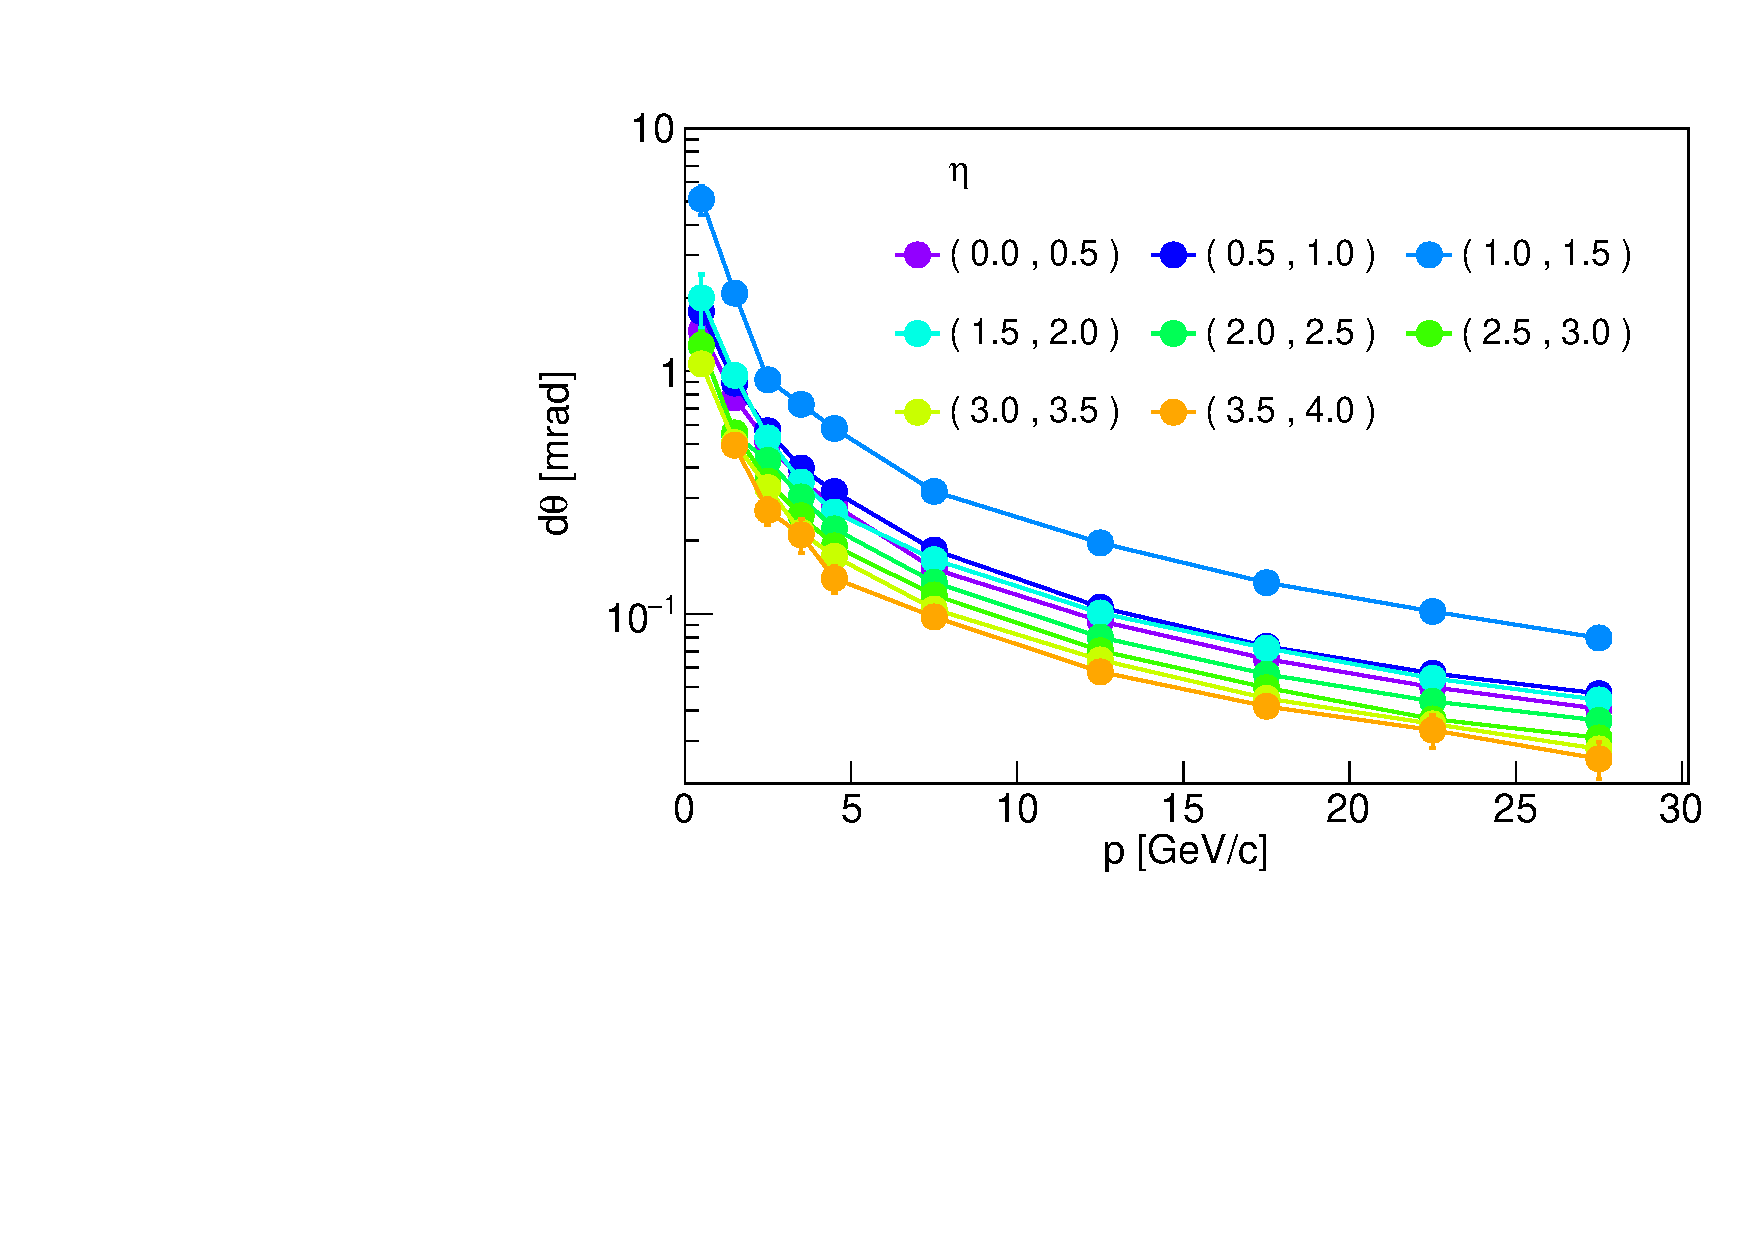
\includegraphics[width=0.45\textwidth, page=1, trim={0 3mm 0 12mm}, clip]{EIC_Jets/results_res_at_PID_10um_separate.pdf}
% %     \includegraphics[width=0.45\textwidth, page=2, trim={0 3mm 0 12mm}, clip]{EIC_Jets/results_res_at_PID_10um_separate.pdf}
% %     \caption{Polar (left) and azimuthal (right) angular resolutions at the location of PID detectors as a function of momentum for several pseudorapidity bins for pions in the BeAST (3.0~T) magnetic field. These distributions are overall insensitive to the magnetic-field intensity.}
% %     \label{fig:ang_res_at_pid}
% % \end{figure}

% Primary vertex resolutions in three dimensions and a first look at tracking efficiency are determined by generating PYTHIA $e$+$p$ events at 18$\times$275 GeV collisions, reconstructing the final-state particles in the full-simulation detector, and fitting the vertex residual distribution with respect to the generated truth vertex with a Gaussian function. Pattern recognition is seeded using truth-track information. As a result, the extracted quantity constitutes a best-case-scenario and is expected to describe the detector performance only in very-low-multiplicity events. These tracking efficiencies obtained from the full simulation were applied in the following performance projection studies through fast simulation.

% % Figure~\ref{fig:fullsim:vtx}, left plot, shows the resulting primary vertex resolution as a function of track multiplicity in events with $Q^{2}>$1 GeV$^{2}$. One can see the event primary vertex resolution is typically $\sim$25$\mu$m at a multiplicity of $\sim$5, the average number of charged particles produced within the acceptance of tracking detectors in these collisions. Figure~\ref{fig:fullsim:vtx} right plot shows the charged pion tracking efficiency in different $\eta$ regions, which shows reasonable tracking efficiencies over a broad kinematic region. 


% \begin{figure}[htbp]
%     \centering
%     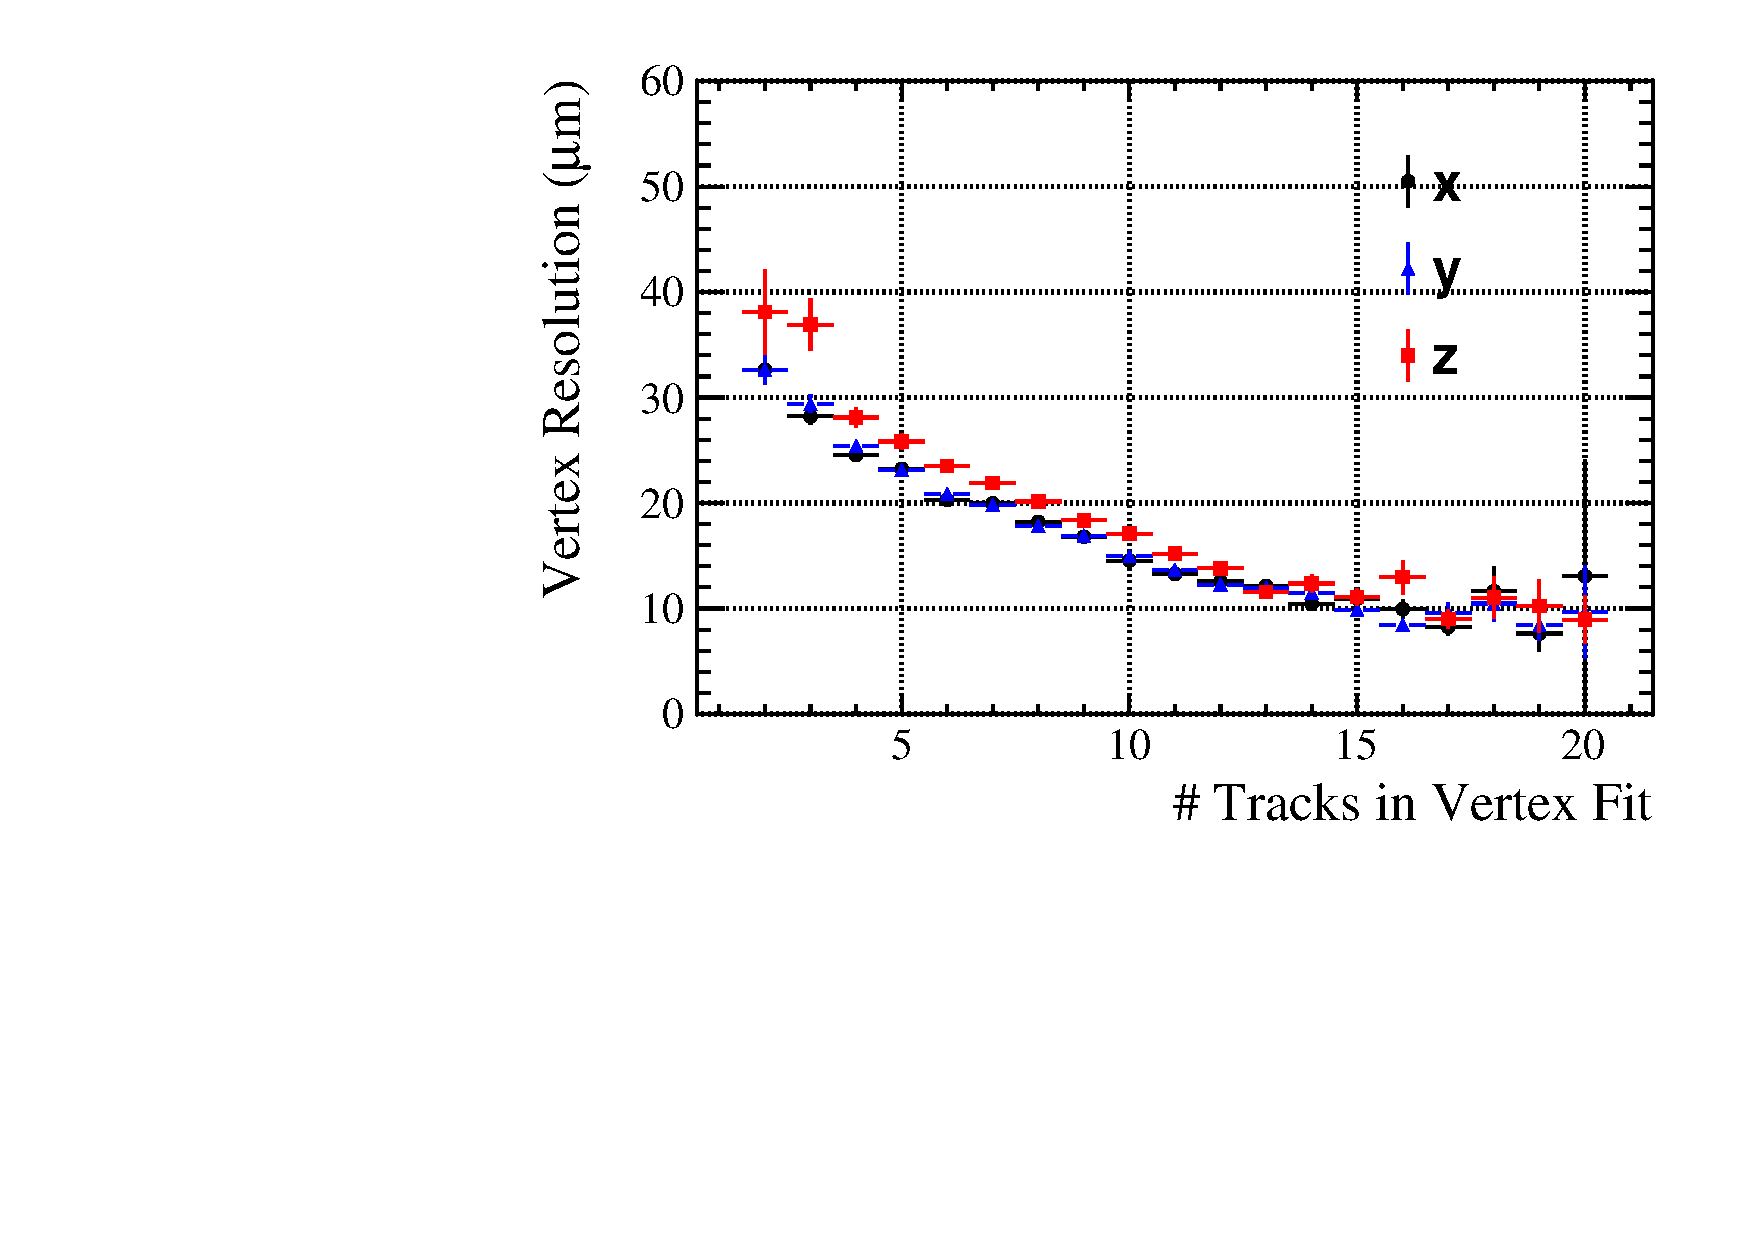
\includegraphics[width=0.45\textwidth]{EIC_Jets/VertexRes.pdf}
%     \hspace{0.2in}
%     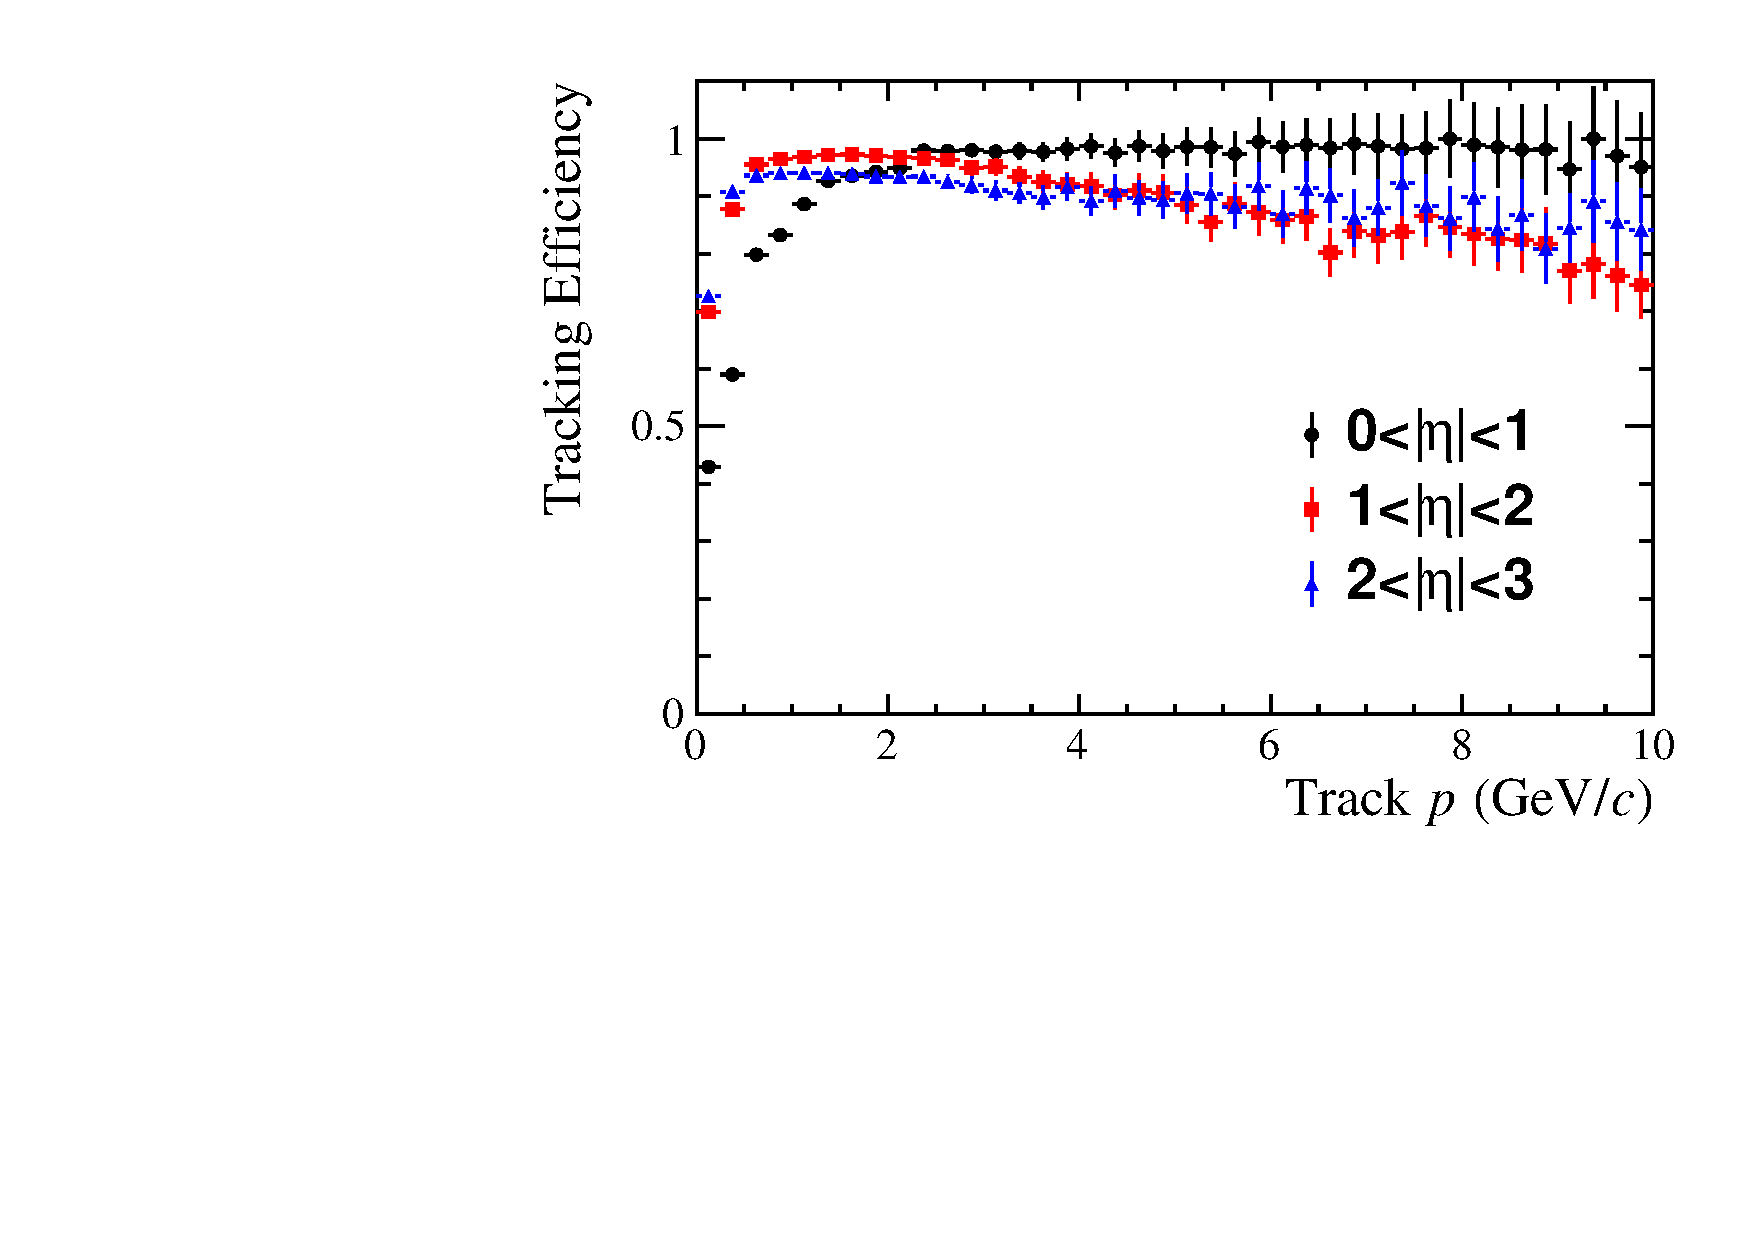
\includegraphics[width=0.45\textwidth]{EIC_Jets/TrackEff.pdf}
%     \caption{Left: primary vertex resolution determined in the full simulation setup with PYTHIA $e$+$p$ events at 18$\times$275 GeV collisions with an event level selection of $Q^{2}>$1 GeV$^{2}$. Right: Tracking efficiency determined in the full simulation for three different $\eta$ regions. Both figures incorporate events generated in a 3.0~T magnetic field.}
%     \label{fig:fullsim:vtx}
% \end{figure}

% Minimum $p_T$ thresholds for the charged particle tracking can be estimated from $p_T[{\mathrm GeV}/c] = 0.3 \cdot B[{\mathrm T}] \cdot r/2[{\mathrm m}]$, derived from Newtonian mechanics.
% Here, $r$ corresponds to the radius of curvature of the track, following a circular trajectory in the magnetic field of intensity $B$. The threshold for a track to reach the outer layer of the detector ($r\geq 43.23$cm) in a 3.0T (1.4T) uniform solenoidal magnetic field corresponds to $p_T \geq$ 195 (90) MeV/$c$ in this estimate. We can consider a lower threshold corresponding to particles that reach the third barrel layer ($r\geq 21.00$cm), since three is the minimum number of hits needed for a momentum reconstruction. Clearly, not reaching the outer layers has a negative impact on the resolution of such particles. In this case, the threshold in a 3.0T (1.4T) uniform solenoidal magnetic field would correspond to $p_T \geq$ 95 (44) MeV/$c$.
% However, energy-loss and multiple scattering, in particular for non-relativistic particles, lead to higher thresholds than the values estimated above. Conservative values for the thresholds in the studies of jets.

% In this section, simulations were carried out with magnetic-field maps
% incorporating a gradual decrease in the magnetic-field strength with increasing distance from the nominal interaction point in the $z$ direction.
% Furthermore, the BaBar magnet, which is a candidate solenoid for the EIC, peaks at $B = 1.4$T. In some of the studies presented in this document, parametrizations from perfectly-solenoidal fields determined for $B = 1.5$T are used.
% The change between $B = 1.4$T and $1.5$T leads to a 7$\%$ difference in the momentum resolution. Additionally, differences between realistic field maps and uniform solenoids lead to $\sim10\%$ differences at high-$|\eta|$. These differences should not affect the conclusions reached in each section.


\section{Jet Physics at the EIC}
As discussed previously, jets are composite objects that relate final-state particles measured in the detector to an initial parton, and serve as a powerful tool for probing QCD. Jets are measured experimentally by clustering the observed particles using a particular clustering algorithm (anti-$k_T$ \cite{Cacciari:2008gp} in this work) within a chosen jet resolution parameter. In heavy-ion collisions, prompt $\gamma$-jet and $\gamma$-hadron correlations are labelled "the golden channel", because the measured photon constrains the kinematics scattered parton, allowing one to study deviations or modifications to the parton more accurately. Such constrains in heavy-ion physics are not common, due to the extremely high multiplicity environments. 

Semi-Inclusive Deep Inelastic Scattering (SIDIS) at the EIC goes much further in this regard, and thus can yield exciting new insights to studying QCD in nuclei. By accurately measuring the energy of the electron before and  after the scattering, one obtains an excellent handle on the momentum that is transferred from the beam electron to the parton. Thus, at leading order, the parton should have momentum $Q$ in the absence of any modification, and yield a measured jet with comparable momentum. Rather than a rare event, as it is in prompt photon channels in heavy-ion collisions, SIDIS events are the rule, not the exception. Figure~\ref{fig:eic_dis} shows a carton of SIDIS with a measured jet. Futhermore, jet can be measured at much lower $Q^2$ at the EIC when compared to the LHC, down to  $Q^2 = 10^{-5}$ \cite{Khalek2021}.

\begin{figure}[htb]
\centering
	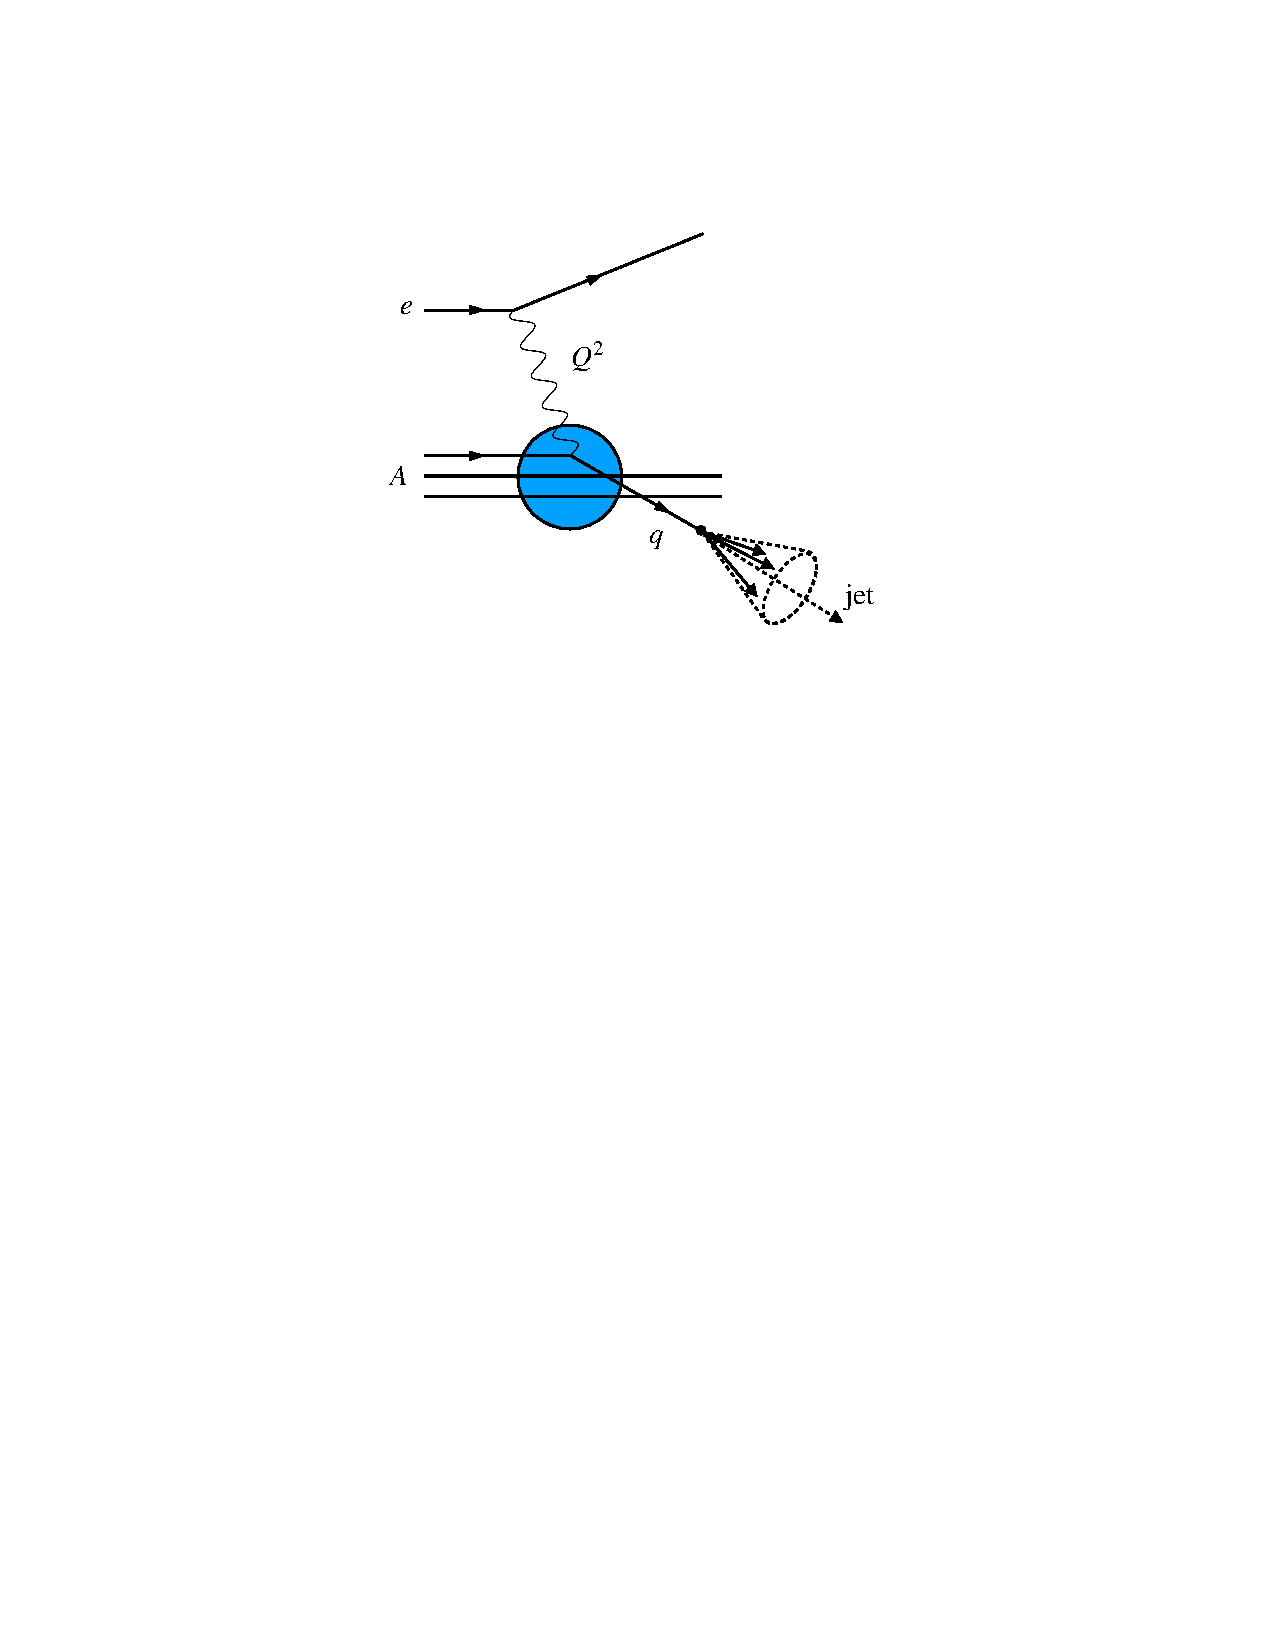
\includegraphics[width = 0.5 \textwidth]{EIC_Jets/LO_DIS_Diagrgram_jet.pdf}
	\caption{Leading order deep inelastic scattering diagram. The struck quark is observed as a jet of final state hadrons and serves as an excellent probe of the nucleus.}
  \label{fig:eic_dis}
\end{figure}

Earlier studies of $e$+$p$ collisions utilized jets, but in a limited fashion \cite{Wong:2020xtc}.
An extensive jet program has been proposed for the EIC, as follows: 
%
\begin{itemize}
\item Jets from electroproduction in DIS can be used to study parton energy loss and interactions in cold nuclear matter~\cite{Arratia:2019vju}.
\item Inclusive jet production in polarized electron-proton collisions constrains the helicity-dependent parton distribution function (PDF) of the proton at low $x$, complementary to existing measurements at high-$x$~\cite{Boughezal:2018azh}. 

\item Inclusive jet production in DIS off nuclei ~\cite{Klasen:2017kwb} and dijet quasi-real photoproduction~\cite{Klasen:2018gtb} can be used to advance our knowledge of nuclear PDFs. 
\item Dijet photoproduction gives access to the photon PDF~\cite{Chu:2017mnm}. \item Single-inclusive lepton scattering resulting in jets, where the scattered electron is not observed, has been proposed as an EIC measurement to study transverse spin effects in the nucleon~\cite{Hinderer:2015hra,Hinderer:2017ntk}.

\item Jets complement measurements of the three-dimensional structure of hadrons, encoded in transverse momentum-dependent (TMD) PDFs and fragmentation functions (TMD FFs).
Unlike in the semi-inclusive DIS case, jet measurements allow the extraction of these two quantities separately. Specifically, jet measurements at the EIC have been proposed to constrain the quark Sivers function, transversity distribution, and the Collins FF~\cite{Arratia:2020nxw}. 
\item Dijet production can be used to access gluon TMD functions at the EIC~\cite{Zheng:2018ssm,Dumitru:2018kuw}.

\item Charm-jet cross section measurements can be used to resolve the tension between different experimental results regarding the strangeness content of the nucleon~\cite{Arratia:2020azl}.

\item Substructure measurements can be used to tune parton-shower event generators and study cold nuclear matter effects as explored in~\cite{Aschenauer:2019uex}.
\end{itemize}

Of particular interest for this work is the study of jets to study parton energy loss that can be observed as a \pt~broadening effect on the measured jet; When a highly energetic jet is produced in the hard partonic process, it experiences multiple interactions with the target nucleus which will generate \pT~-broadening effects \cite{Baier1997}. These final state interactions can also be factorized into the TMD quark distribution of the nucleus, from which one can extract the typical transverse momentum obtained by the quark, $\hat{q}L$, through multiple interactions with the cold nuclear matter\cite{Liang2008a}.  The \pt~broadening effect can be observed by measuring electron jet correlations, and modelled using different $\hat{q}L$. This is shown in Fig.~\ref{fig:ql_corr}.

\begin{figure}[htpb]
  \centering
  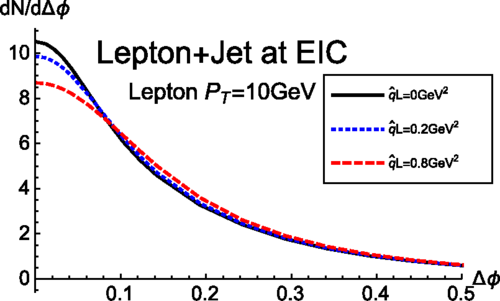
\includegraphics[width=0.6\textwidth]{EIC_Jets/qL_corr.png}
  \caption{\pt~broadening effects  for the lepton jet azimuthal correlation due to the interaction with cold nuclear matter as a function of $\Delta\varphi = |\varphi_\mathrm{jet} - \varphi_{l} - \pi|$ for two typical values of $\hat{q}L$ \cite{Liu2019}.}
  \label{fig:ql_corr}
\end{figure}

In the next, section the jet momentum and angular resolutions achievable with the all-silicon tracker are discussed.
%bvj Subsequently, 
Finally, two specific observables, electron-jet correlations in DIS and the charged jet fragmentation function, will be presented to illustrate potential of the physics with jets reconstructed in the silicon tracker. 


\section{Charged Jet Reconstruction Performance}

Of course, the jet physics program at the EIC can only be accomplished with accurate measurements of the final state jets. This section discusses the jet reconstruction performance of the all-silicon tracker described in Sec.~\ref{sec:sim:full}. Charged jets have been measured extensively in $p$+$p$ collisions with the ALICE detector at the large hadron collider~\cite{PhysRevD.91.112012}.
%bvj Before journal submission, let's check what ATLAS did and add a reference if appropriate.

Track-only jets can often offer greater experimental precision, but are traditionally harder to compare to theoretical calculations. However, there has been progress in connecting experimental track-only jet observables with theoretical studies~\cite{PhysRevD.88.034030}. To quantify the jet reconstruction performance of the silicon tracker described in section~\ref{sec:sim:full}, electron-proton collisions are simulated with the PYTHIA8 Monte-Carlo generator and a full GEANT4 simulation with a 1.4 T and 3.0 T solenoidal magnetic field. Electrons and protons are collisions are simulated with a center-of-mass energy of $\sqrt{s}=89$ GeV and a minimum $Q^2$ of  $16(\GeVc)^2$. Jets are reconstructed using the anti-$k_\mathrm{T}$ algorithm, with a large resolution parameter of $R= 1.0$. This is feasible due to the relatively low multiplicity of particles produced in $e$+$p$ collisions. 

Reconstructed jets are required to have 4 or more constituents and a minimum total energy of $4.0~\mathrm{GeV}$ (informed by the minimum $Q^2$ of $16(\GeVc)^2$) in order to be considered. Jets are reconstructed in the range $|\eta|<3.5$, according to the acceptance of the all-silicon tracker. Reconstructed jets within $\Delta R = 0.5$ of the highest energy electron in the event are omitted to ensure that the beam electron is not included as part of any jet.

% ES
Additional selections are made on the jet constituents. They are required to have a $p_\mathrm{T} \geq$ 70 MeV/$c$, with a higher threshold depending on $\eta$ of the constituent. The minimum $p_\mathrm{T}$ for different $\eta$ regions is shown in Table~\ref{tab:min_pt1}. The values in Table \ref{tab:min_pt1} are extracted from Ref.~\cite{DMtable:2020} and exceed the values discussed in section~\ref{sec:sim:full}. These are based on the need for three or more traversed barrel layers or disks in the all-silicon tracker in order to determine the track curvature for a charged particle and hence its transverse momentum. Jets with constituents that hit the conical supports where the central barrel meets the forward and backward disks are omitted. Based on Fig.~\ref{fig:material}, we take this range to be $1.06 < |\eta| < 1.13$.

\begin{table}[htb]
  \centering
\caption{Minimum $p_\mathrm{T}$-threshold (in MeV/$c$) for charged jet constituents.}
\resizebox{\textwidth}{!}{\begin{tabular}{  c | c | c | c | c | c  }
~~$B$ field [T]~~& ~~$ |\eta| < 1.0 $~~ & ~~$ 1.0 < |\eta| < 1.5  $~~ & ~~$1.5 < |\eta| < 2.0 $~~ & ~~$ 2.0 < |\eta| < 2.5 $~~ & ~~$2.5 < |\eta| < 3.5$~~\\
\hline \hline
1.4 & 200 & 150 & 70  & 130  & 100 \\
3.0 & 400 & 300 & 160  & 220  & 150 \\
\end{tabular}}
\label{tab:min_pt1}
\end{table}

Reconstructed jets are matched to truth-level jets by requiring that the two axis of the jet are within $\Delta\mathrm{R} < 0.01$. In the event that two or more truth-level jets satisfy this criteria, the truth jet with the higher energy is matched to the reconstructed jet.
%
Once the jets are matched, the neutral components from the truth-level jets are subtracted to obtain charged truth jets. 
The 4-momenta of the neutral constituents are subtracted from the particle-level generated jets to obtain charged jet 4-vector:
\begin{equation}
\label{eq:neutral_subtraction}
p^{{jet, \ }\mu}_{\mathrm \ charged} = p^{{jet, \ }\mu}_{\mathrm \ total}  - p^{{jet, \ }\mu}_{\mathrm \ neutral}.
\end{equation}
%
Certain aspects of the original jet will be unaltered by the subtraction; the jet area, for example is not recalculated according to Eq.~\ref{eq:neutral_subtraction}. 
%bvj However, a 
A negligible difference was found in the jet performance studies using particle-level jets that were originally charged-only, versus particle-level jets where the neutral components are subtracted.

\begin{figure}[htbp]
    \centering
    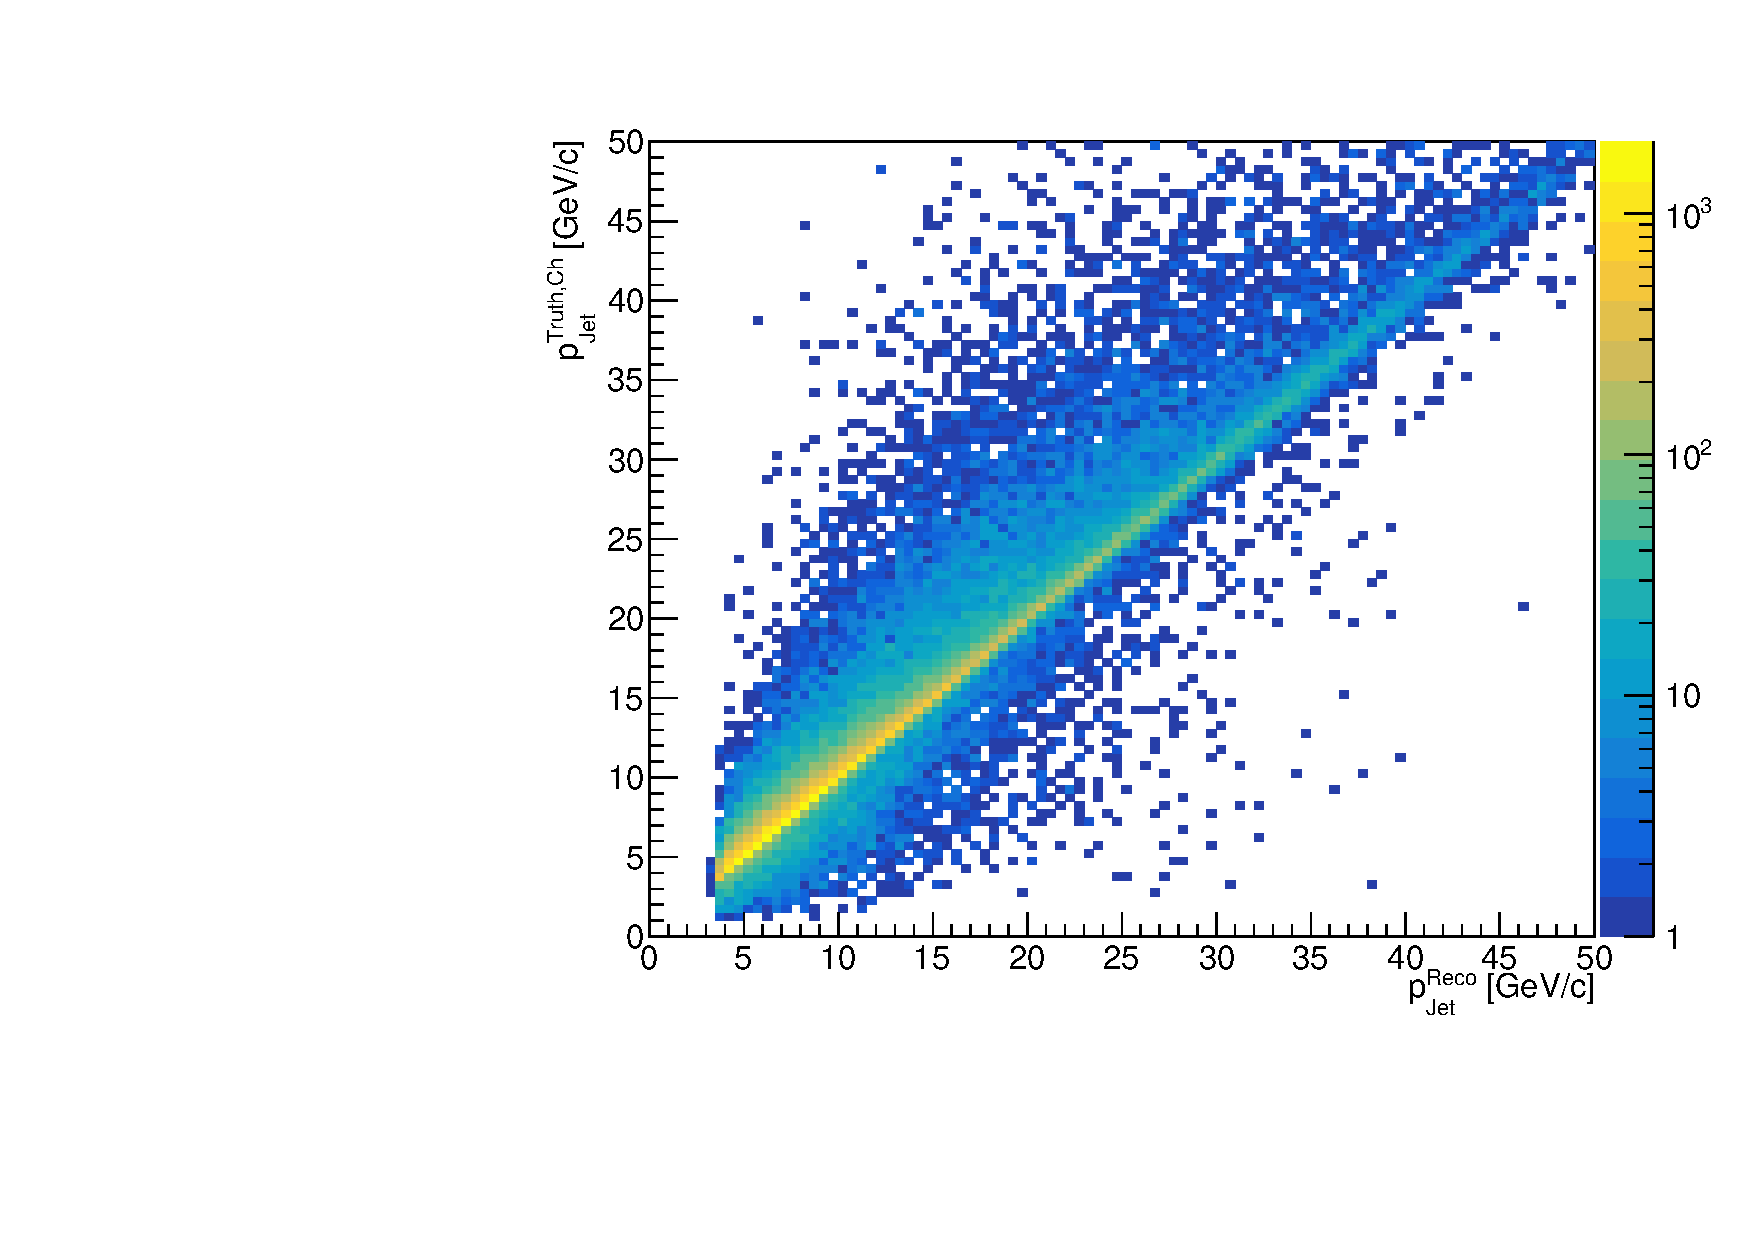
\includegraphics[width=0.49\textwidth]{EIC_Jets/1.4T_momentum_response.pdf}
    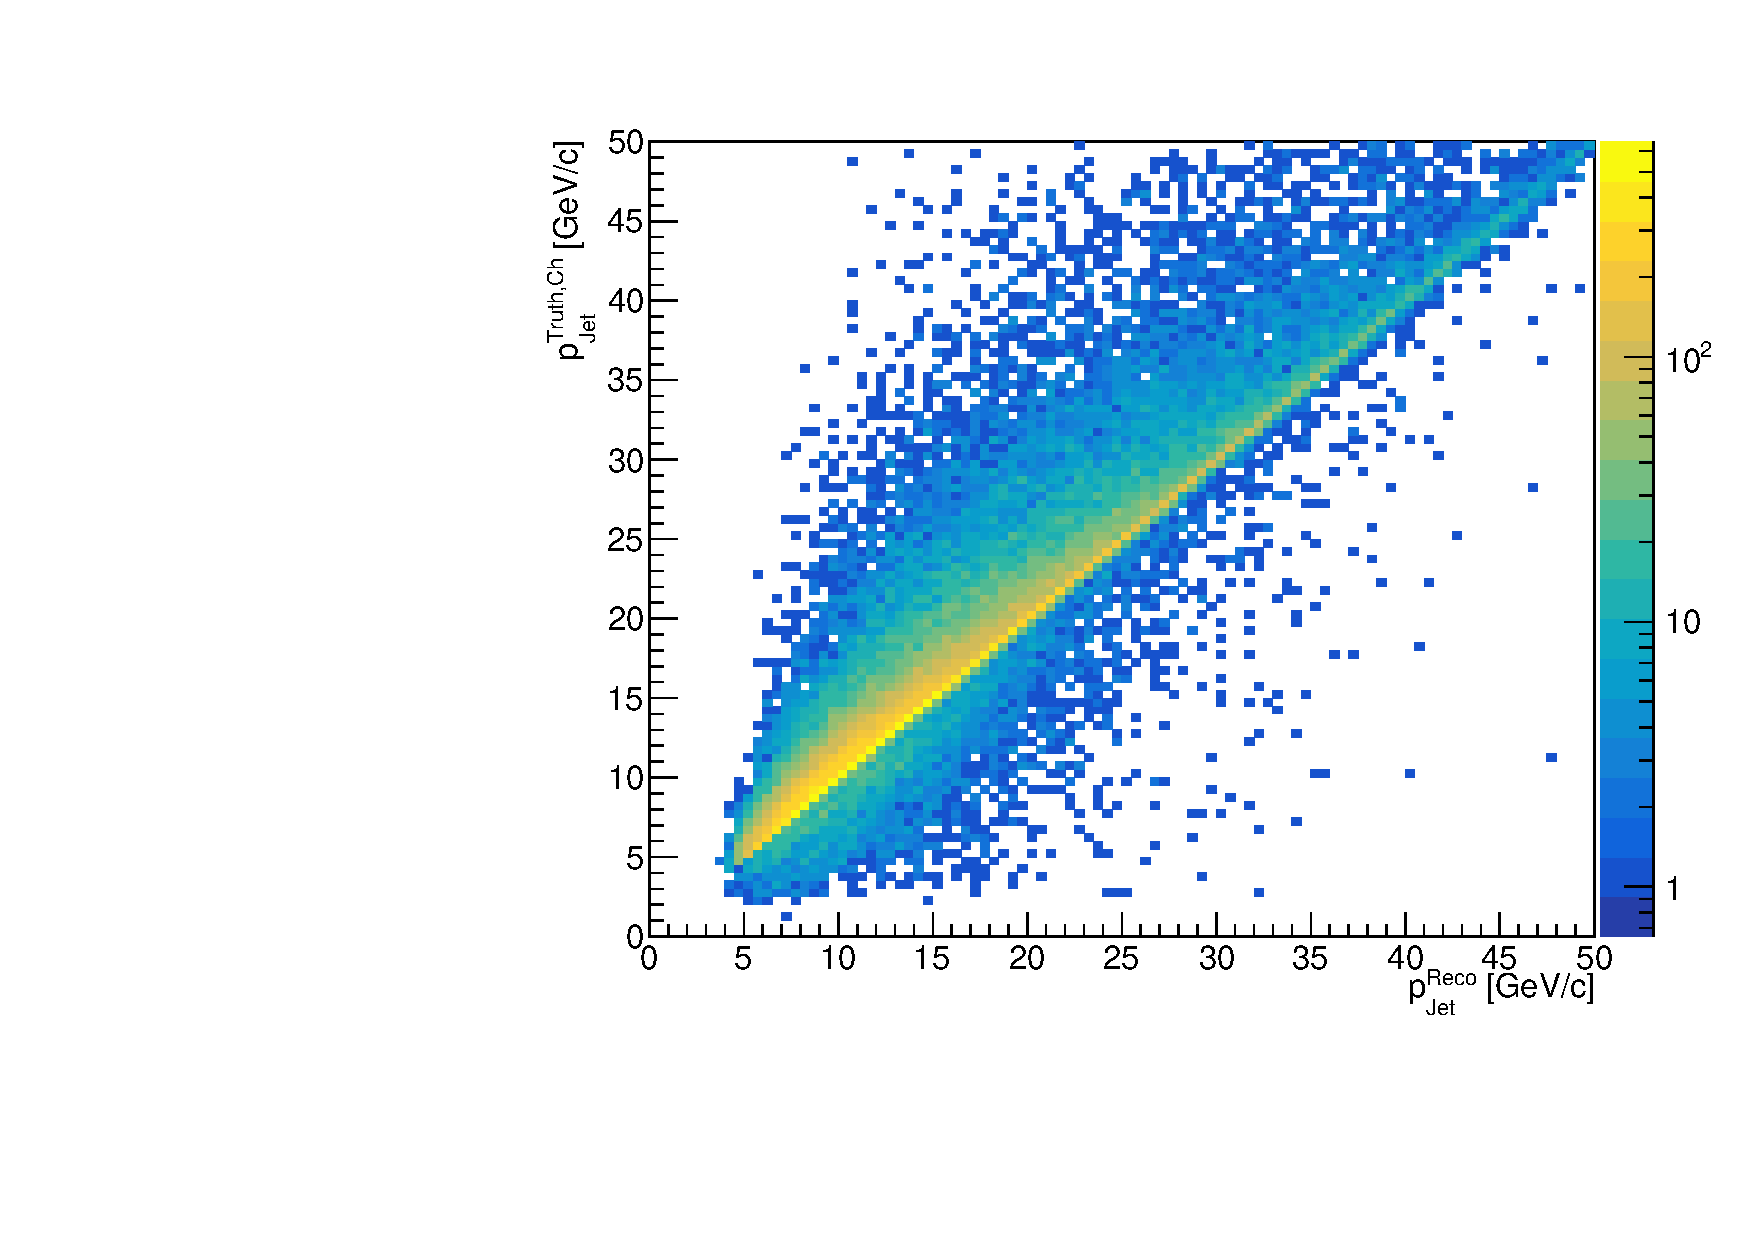
\includegraphics[width=0.49\textwidth]{EIC_Jets/3T_momentum_response.pdf}
    \caption{Charged-jet momentum response for jets with $N_\mathrm{constituent} \geq 4$ determined from PYTHIA $e$+$p$ events at 20$\times$100 GeV collisions in a 1.4 T (left) and 3.0 T (right) magnetic field.}
    \label{fig:jet_response}
\end{figure}

Figure~\ref{fig:jet_response} shows the momentum response matrix for charged jets passing all criteria, with $p_T \ge$ 4 GeV/$c$. There is a strong correlation between the reconstructed jet momentum, $p_\mathrm{Jet}^\mathrm{Reco}$, and the charged truth jet momentum, $p_\mathrm{Jet}^\mathrm{Truth,Ch}$, indicated by the prominent diagonal line in the histogram. There are, however, jets that fall outside of this strong linear correlation. The most important variable impacting the energy and position resolution of jets after all other selections are made is the number of particles not reconstructed as part of the jet (ie ``missing'' particles).

\begin{figure}[htbp]
    \centering
    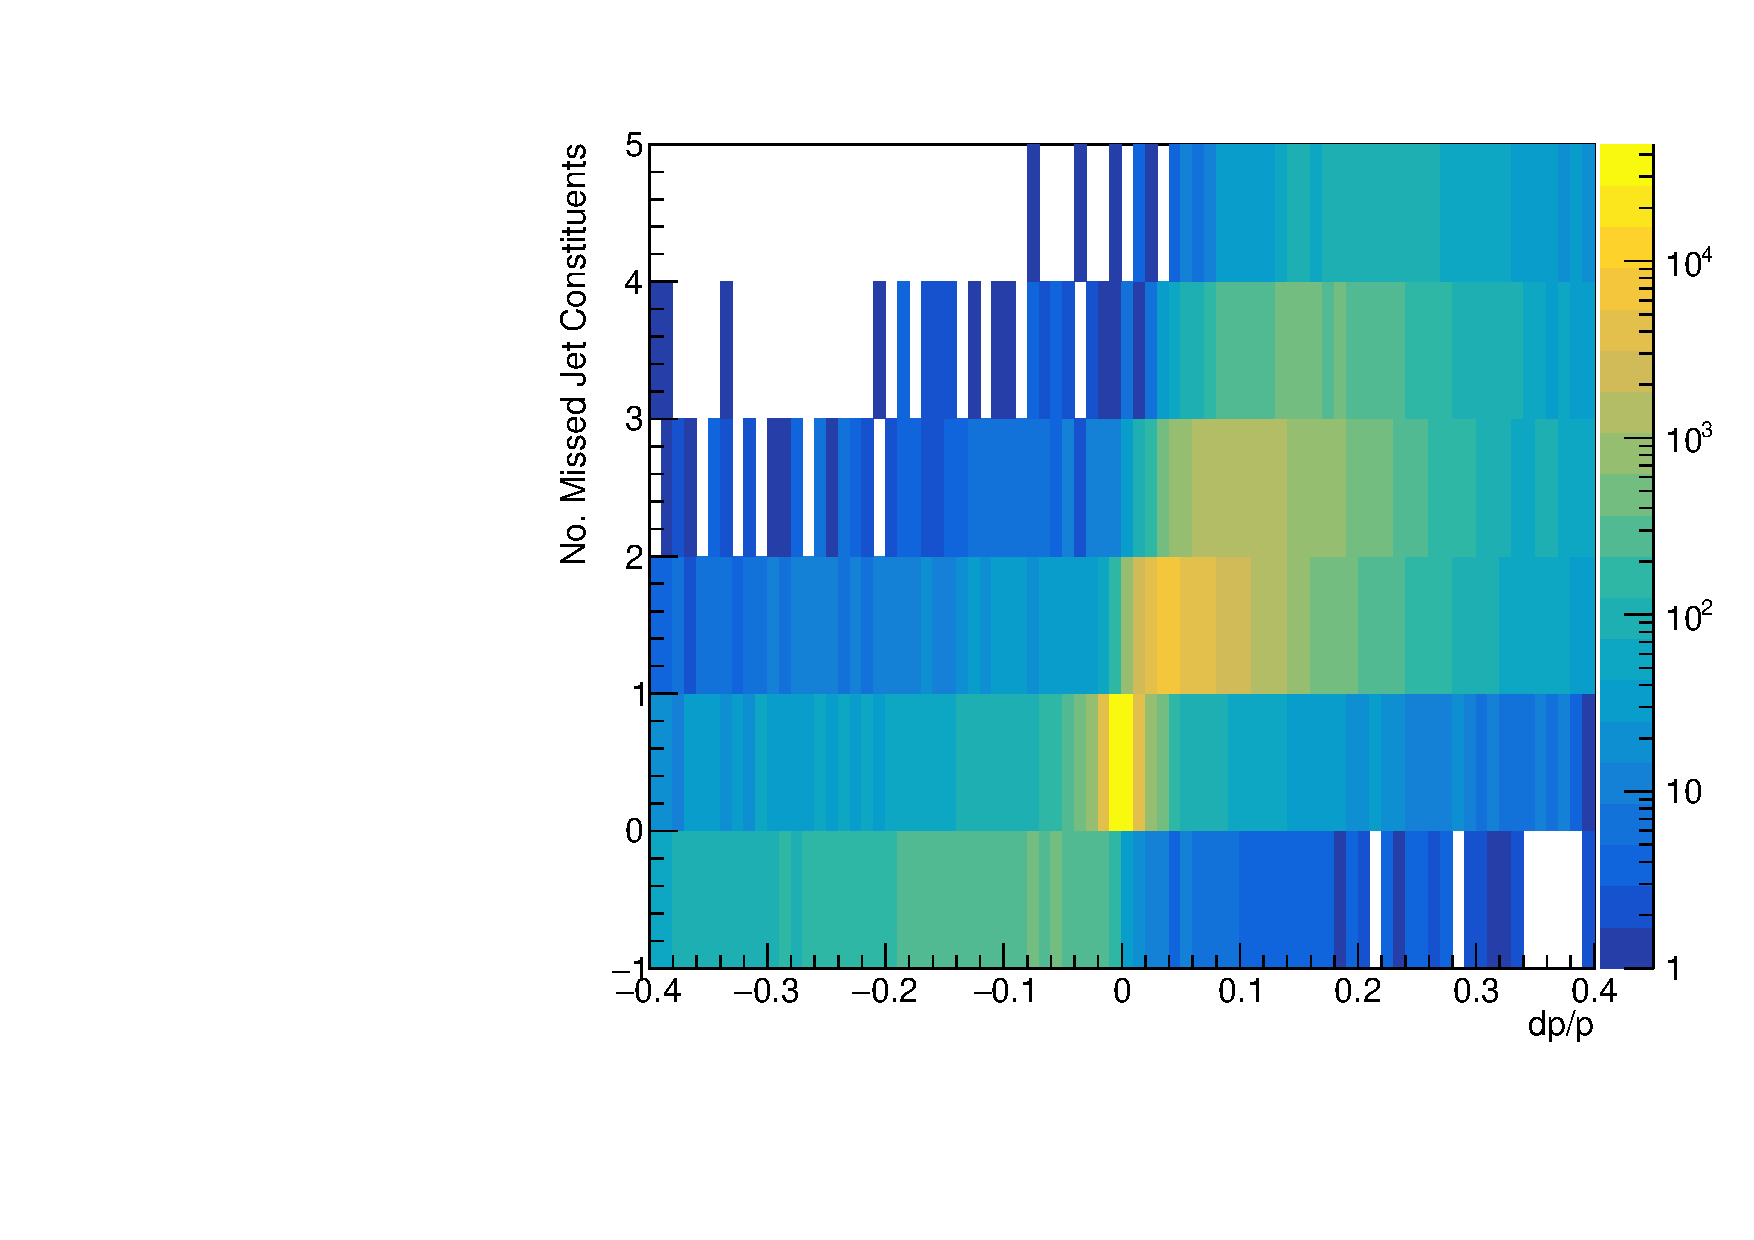
\includegraphics[width=0.42 \textwidth]{EIC_Jets/N_Miss_dPP}
    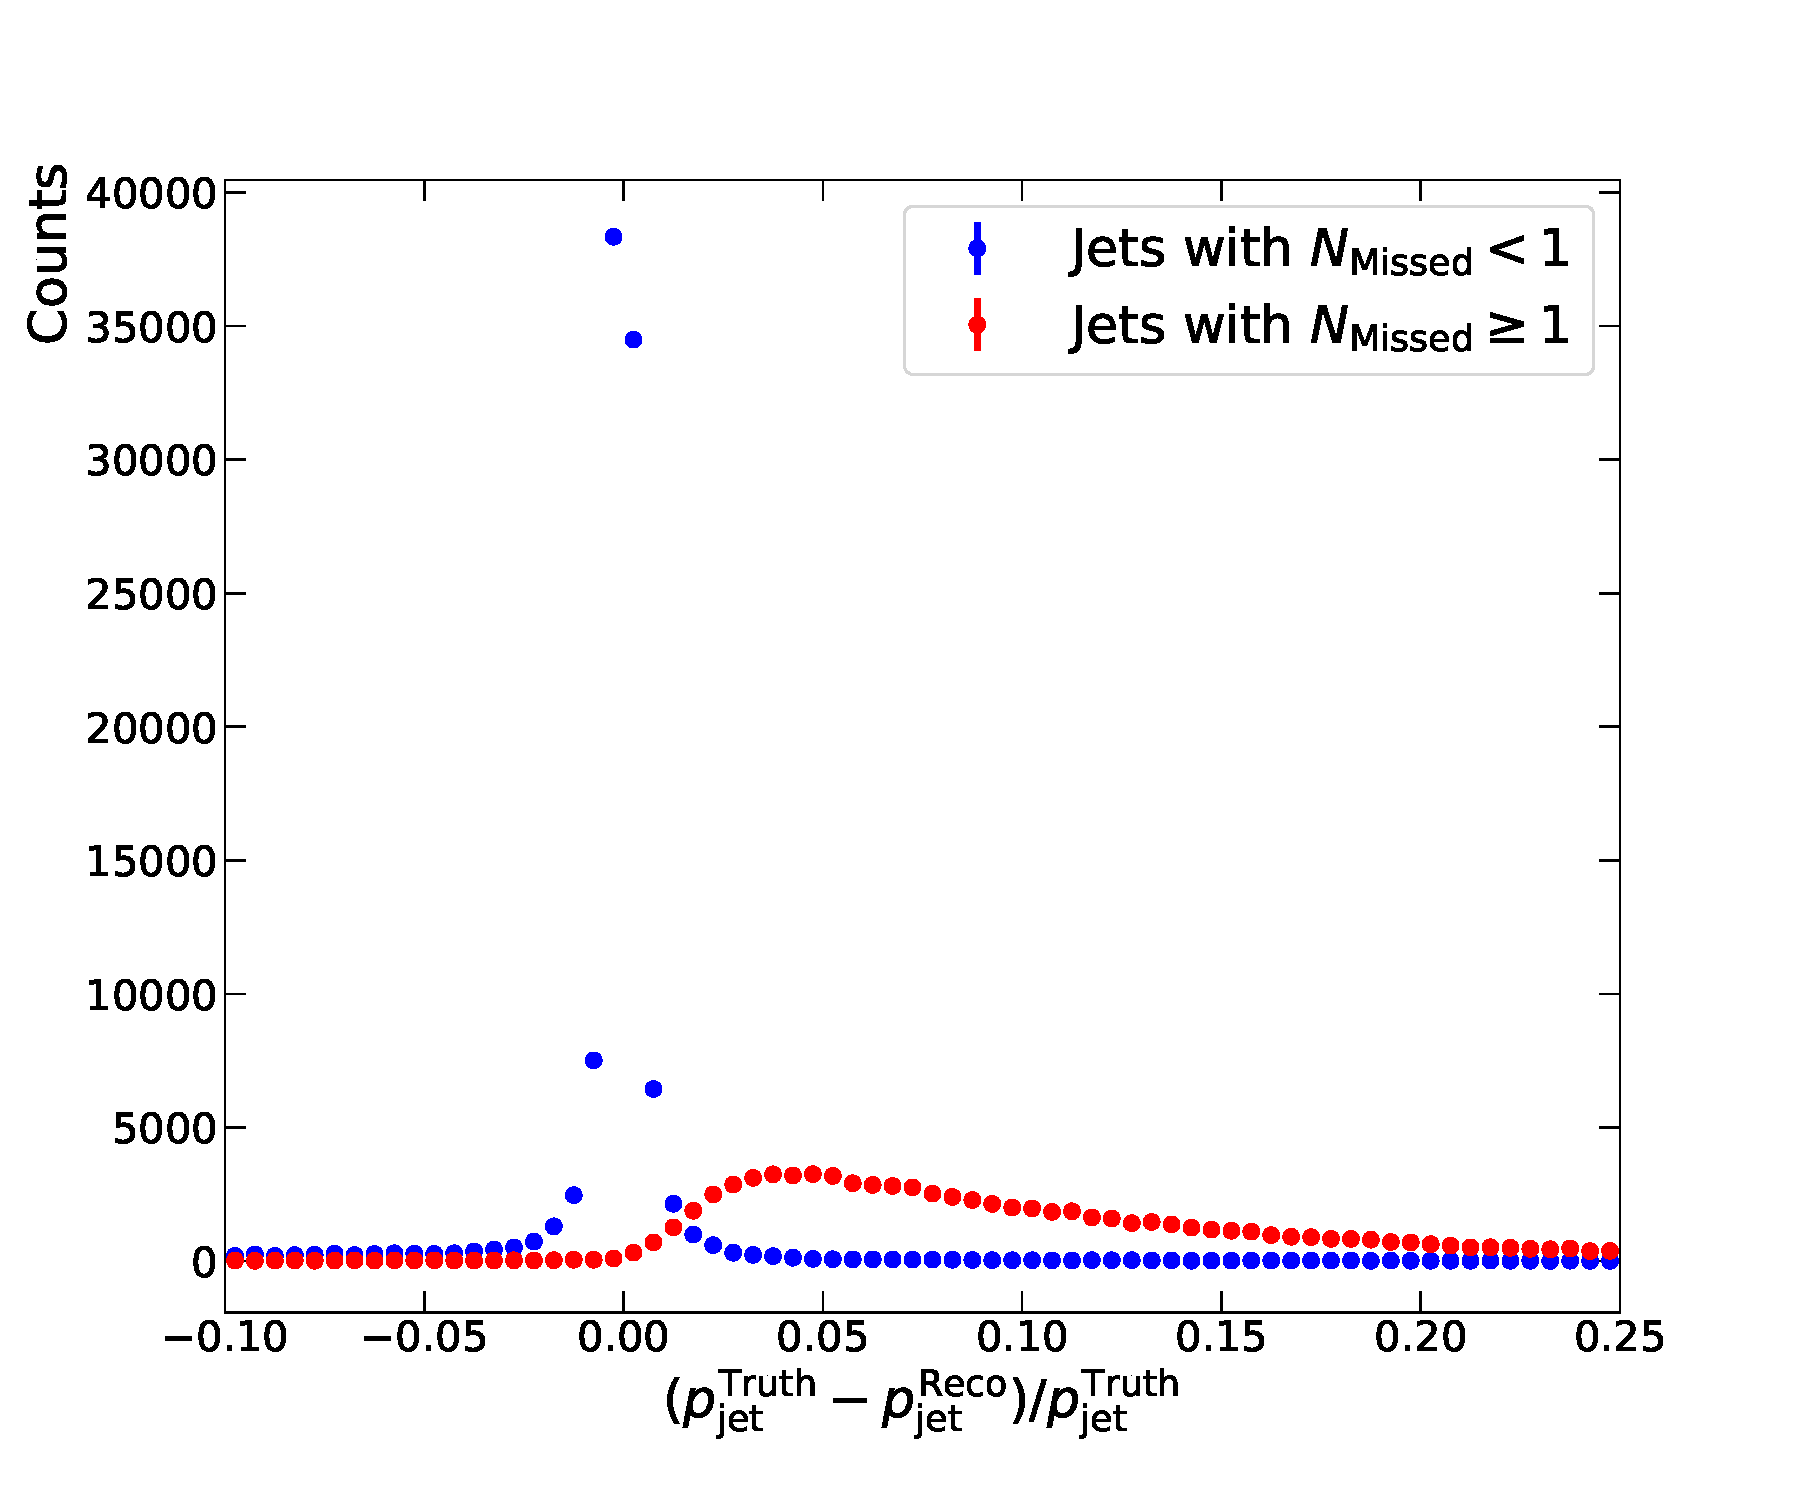
\includegraphics[width=0.42 \textwidth]{EIC_Jets/dPP_two_jets}
    \caption{(Left) Number of missed jet constituents ($N_\mathrm{constituent}^\mathrm{truth} - N_\mathrm{constituent}^\mathrm{reco})$ vs. Jet d$p/p$. (Right) d$p/p$ distribution of jets with less than 1 missing constituent (blue), and jets with with one or more missing constituents (red).}
    \label{fig:n_missed_vs_dpp}
\end{figure}

Figure~\ref{fig:n_missed_vs_dpp} shows the energy resolution of jets vs. the difference between number of truth and reconstructed constituents, $N_\mathrm{Missed} = N_\mathrm{constituent}^\mathrm{truth,ch} - N_\mathrm{constituent}^\mathrm{reco}$. 
The left panel shows a distribution centered at 0 for jets with no missing constituents. As the number of missed jet constituents increases, this distribution broadens and shifts towards higher values of d$p/p$. The right panel shows the d$p/p$ distribution of two populations of jets: jets with less than 1 missing constituent and jets with one or more missing constituents. Jets in a magnetic field of 1.4 T (3.0 T) with less than 1 missing constituent make up approximately 58\% (49\%) of jets that pass all other selection criteria and have a narrow distribution centered at 0 that is well described by a Gaussian fit. Jets with one or more missing constituents, however, have a much broader d$p/p$ distribution that is shifted toward higher values. These are best described by a Landau distribution. Consequently, we characterize the jet momentum resolution of the silicon tracker by simply taking the standard deviation of the d$p/p$ distribution; 
%bvj as 
Gaussian fits to the combined distributions are dominated by the narrow peak at d$p/p$ $\approx$ 0, with the detrimental effect of poorly characterizing the non-Gaussian ``shoulder'' shown in red in Fig.~\ref{fig:n_missed_vs_dpp}.


\begin{figure}[htbp]
    \centering
    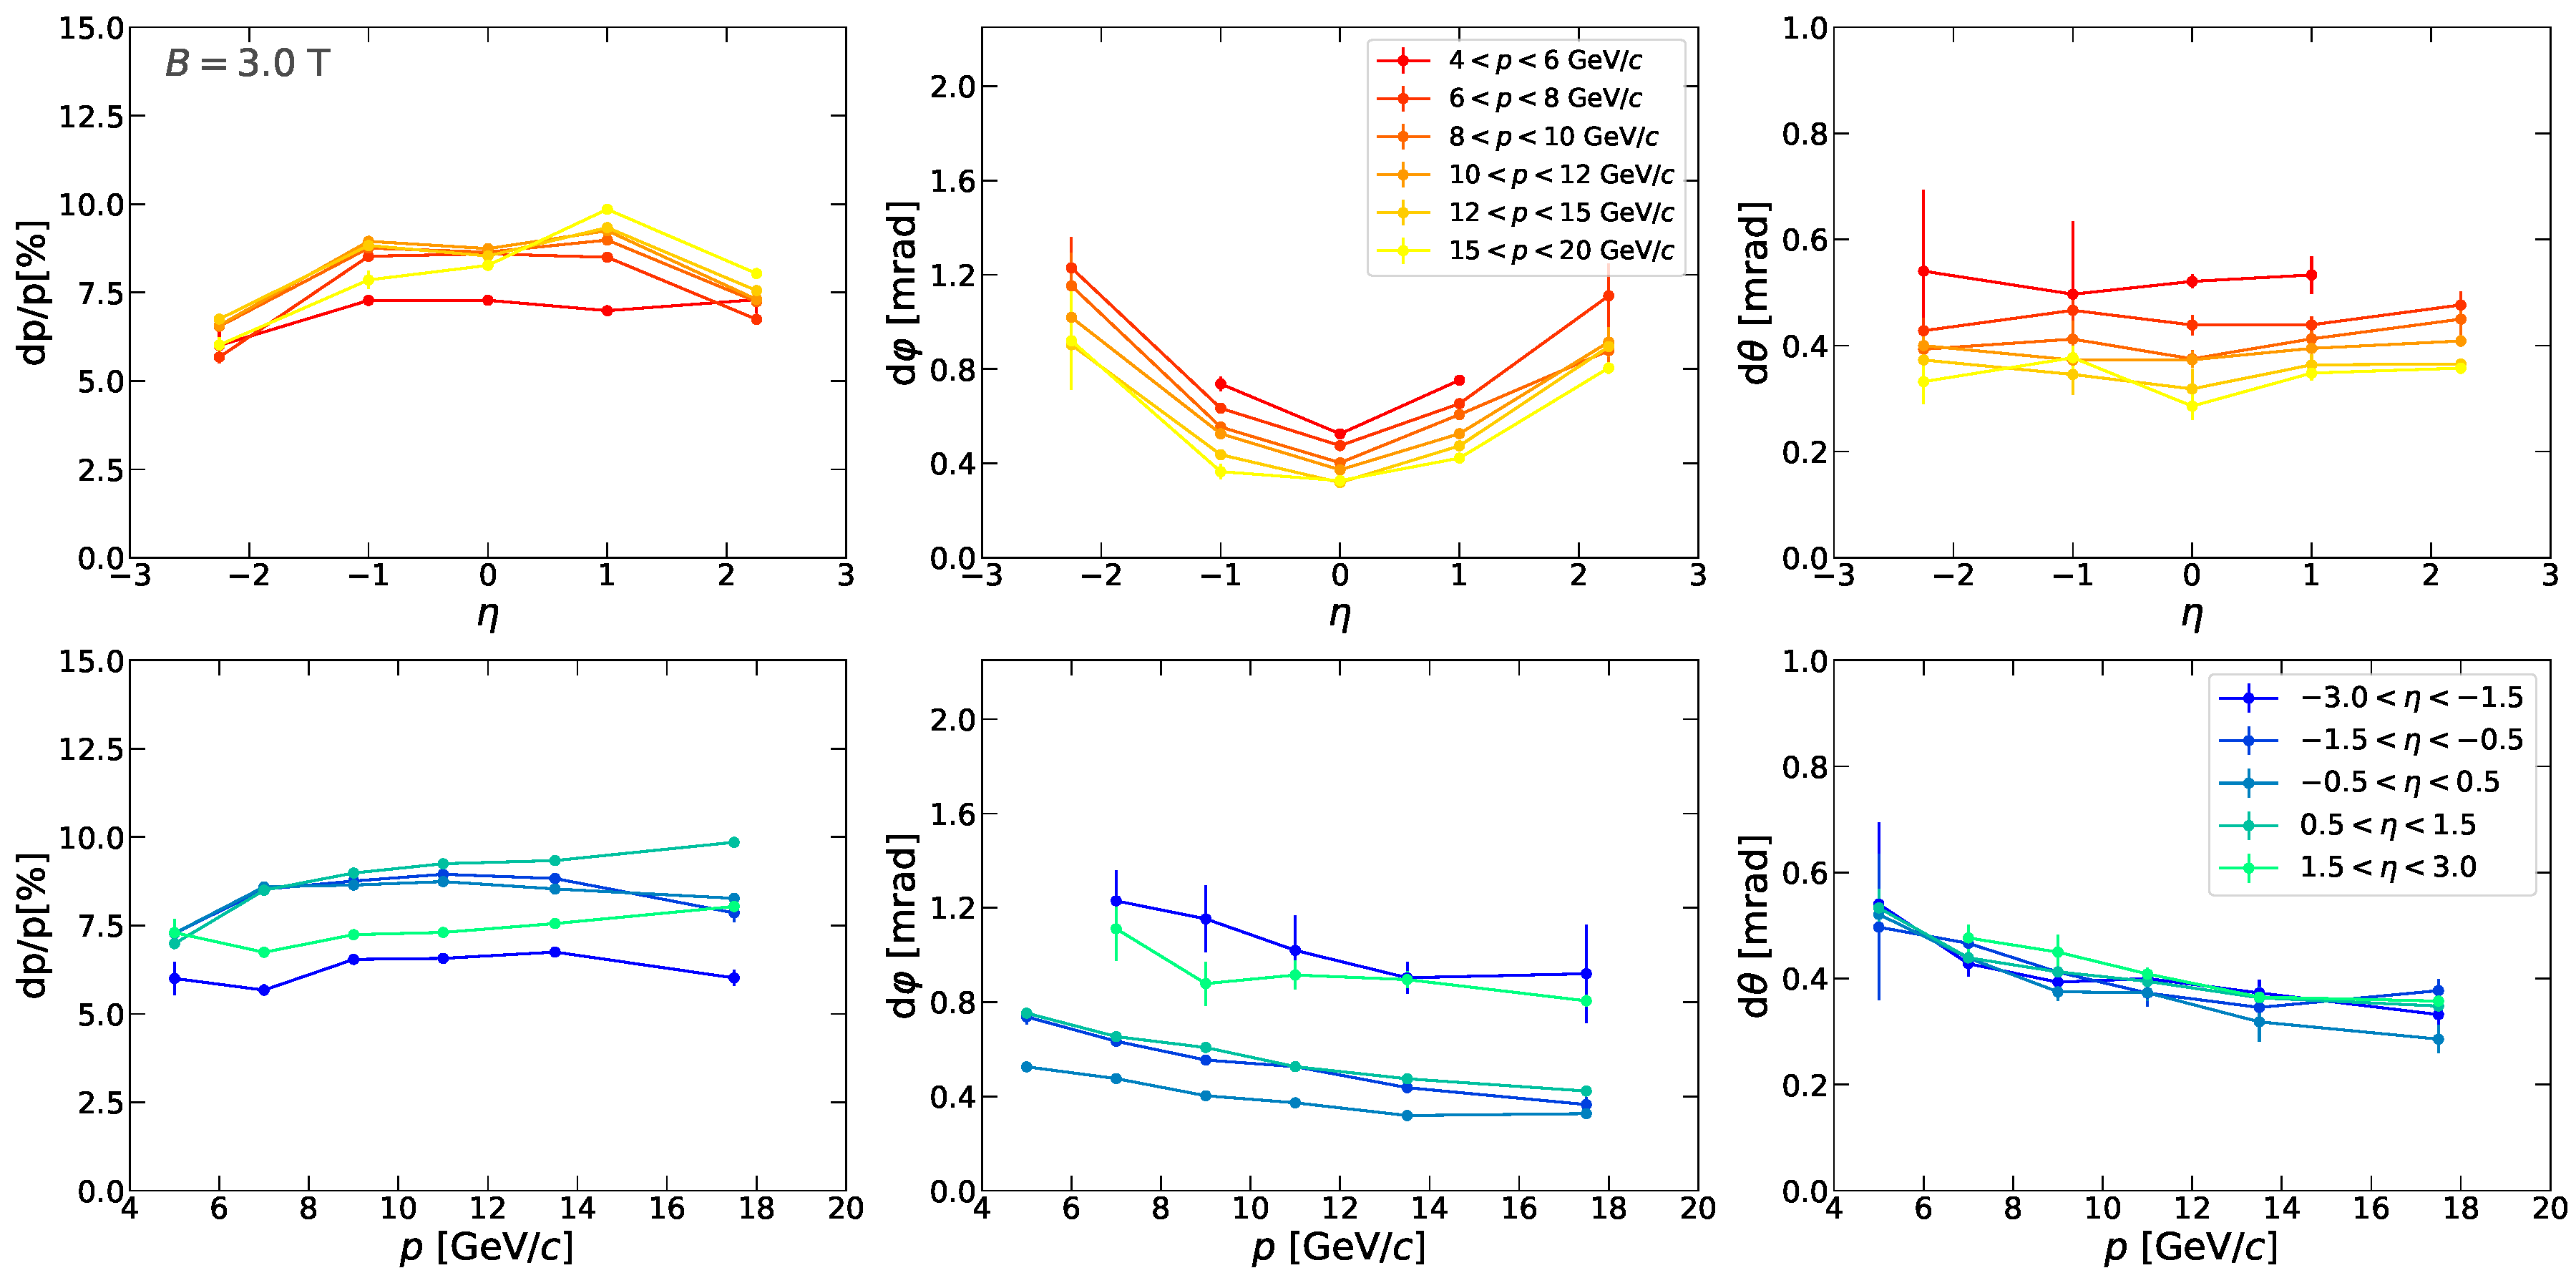
\includegraphics[width=0.96\textwidth]{EIC_Jets/DeltaR_B_3.0_resolutions_eta_mom.pdf}
    \caption{Momentum and angular resolutions of charged jets, reconstructed with the all-Silicon tracker simulated in PYTHIA $e$+$p$ collisions at 20$\times$100 GeV with the 3.0T magnetic-field configuration.}
    \label{fig:3T_jet_resolutions}
\end{figure}

\begin{figure}[htbp]
    \centering
    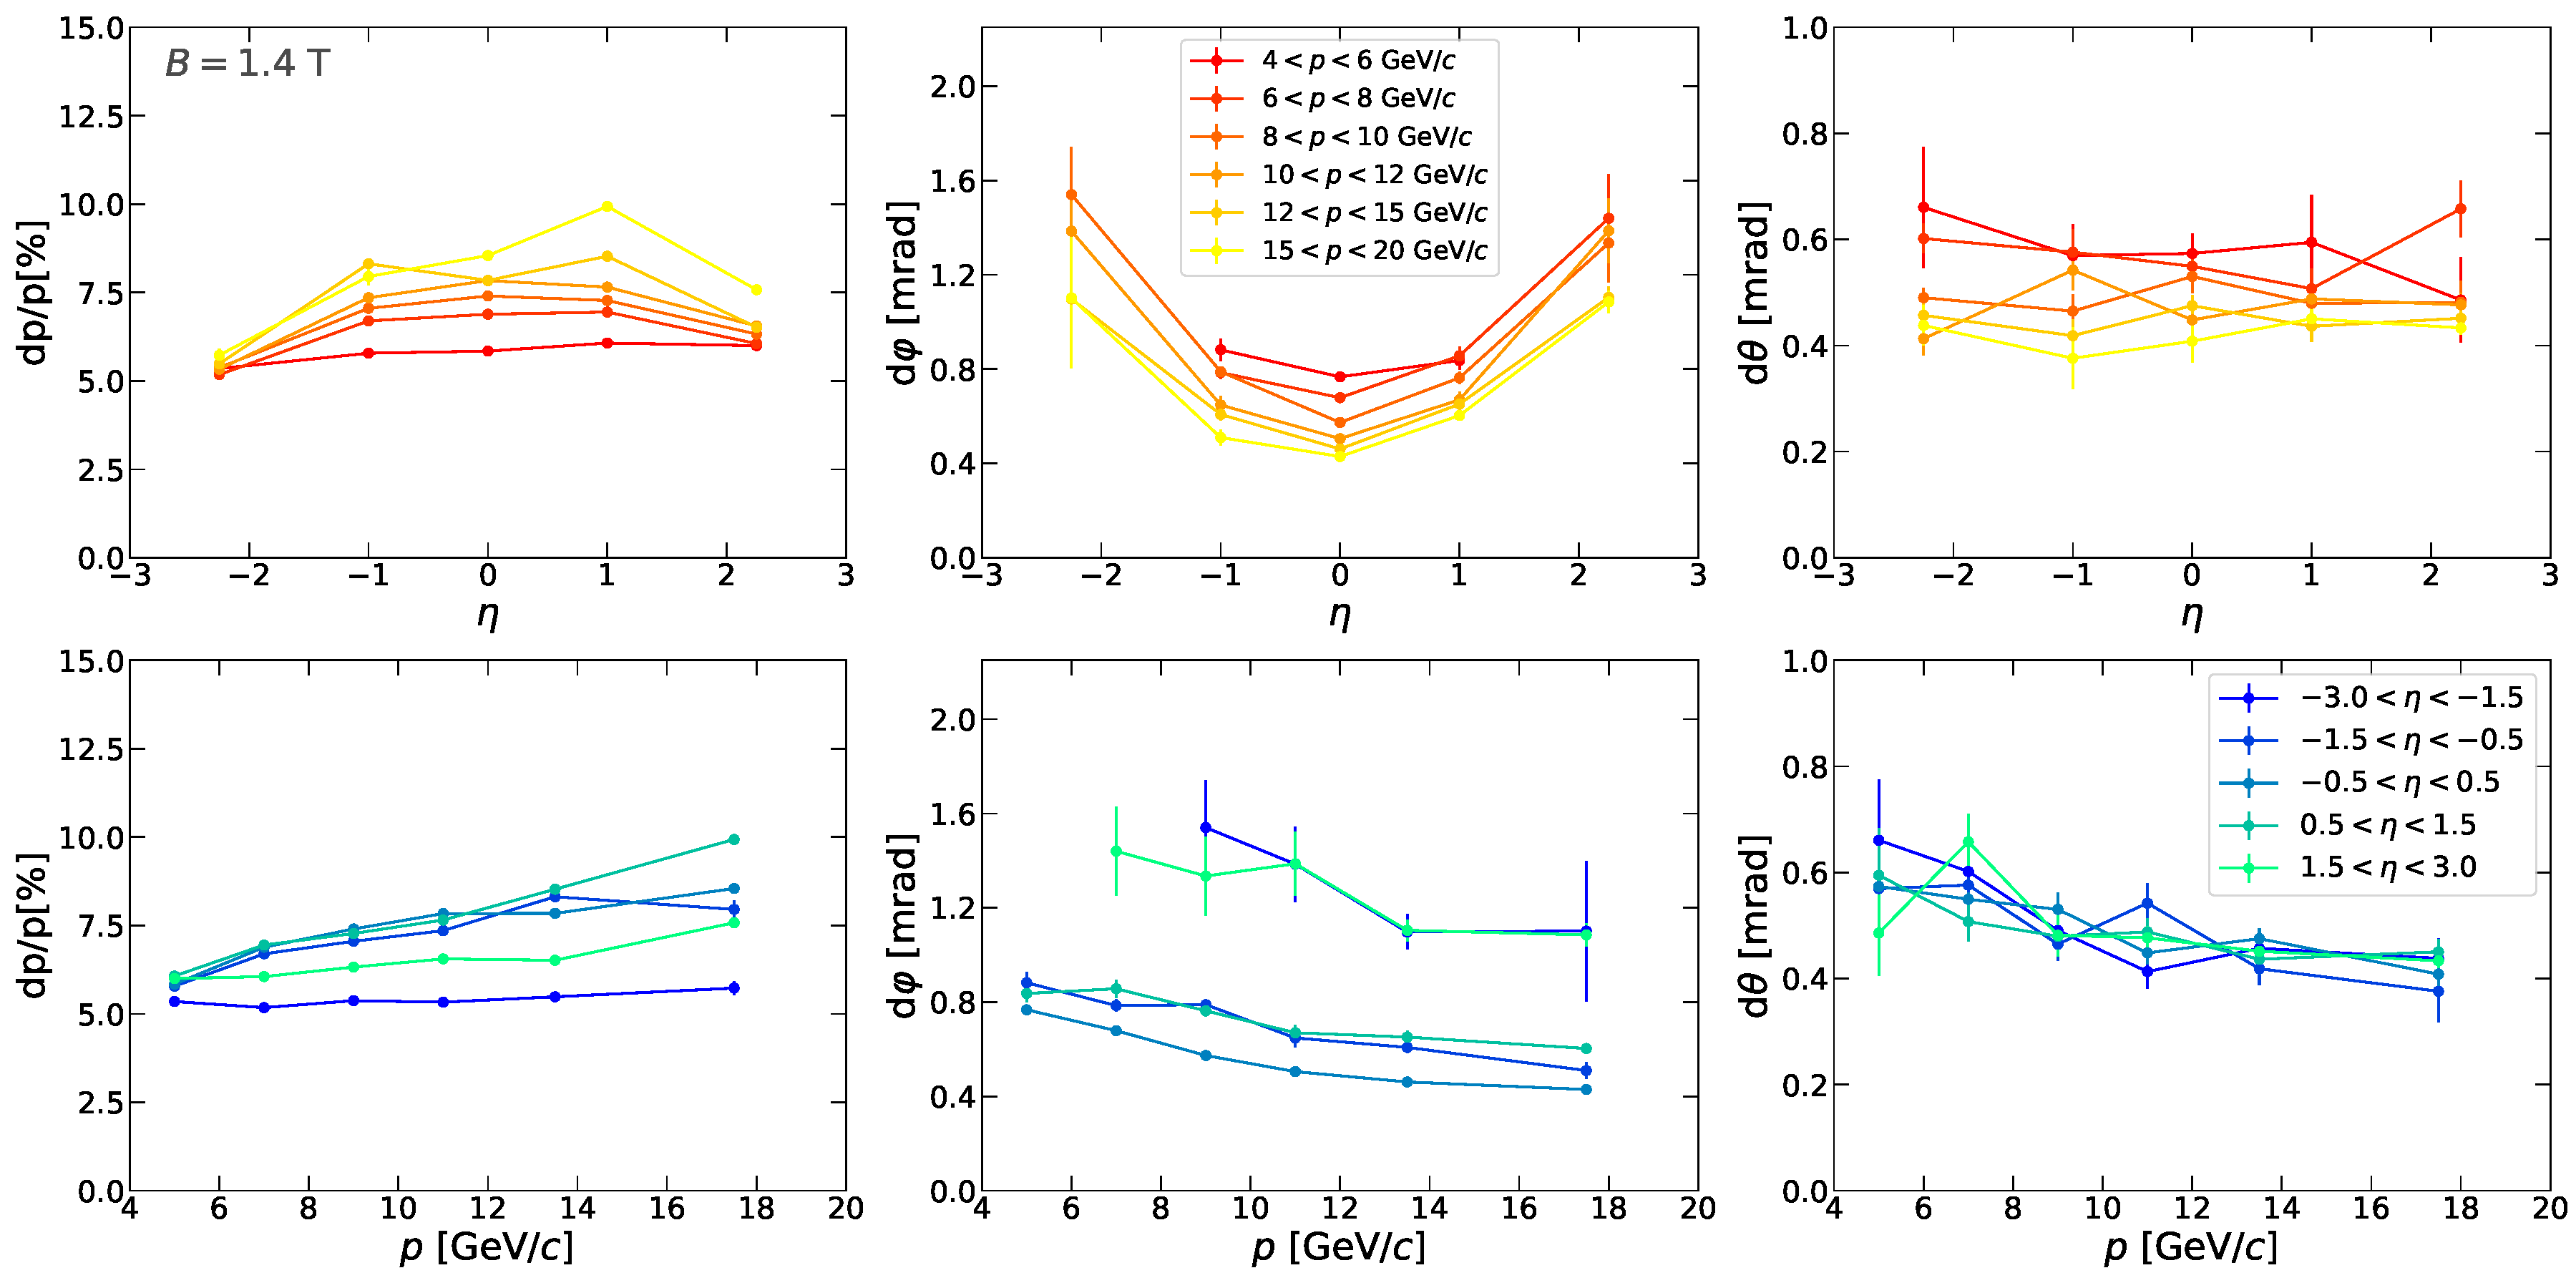
\includegraphics[width=0.96\textwidth]{EIC_Jets/DeltaR_B_1.4_resolutions_eta_mom.pdf}
    \caption{Momentum and angular resolutions of charged jets reconstructed with the all-Silicon tracker simulated in PYTHIA $e$+$p$ collisions at 20$\times$100 GeV with the 1.4 T magnetic-field configuration.}
    \label{fig:1p4T_jet_resolutions}
\end{figure}

Figure~\ref{fig:3T_jet_resolutions} shows the momentum and angular resolutions of jets in a 3.0 T field. The resolutions are shown in bins of jet momentum and $\eta$. The momentum resolution for jets with one or more missing particles that make up the shoulder of the distribution is more difficult to describe. The d$p/p$ distribution shown in Fig.~\ref{fig:n_missed_vs_dpp} in red is best fit with a Landau distribution, where $\sigma$ is undefined. Therefore, instead of a fit, the simple numerical standard deviation of the overall distribution is taken, and reported for the momentum resolution in Fig.~\ref{fig:3T_jet_resolutions}. The angular resolutions are well described by double-Gaussian fits, where in both the azimuthal and polar angular distributions there is  a narrow peak centered at zero, with a low shoulder at larger values. The narrow Gaussian from the fit  is used to the standard deviation and its uncertainty is estimated from the fit. Figure \ref{fig:1p4T_jet_resolutions} shows the resulting resolutions of applying this procedure to jets simulated in a 1.4 T magnetic field.


\section{Charged Jet Observables at the EIC}

\begin{figure}[htbp]
    \centering
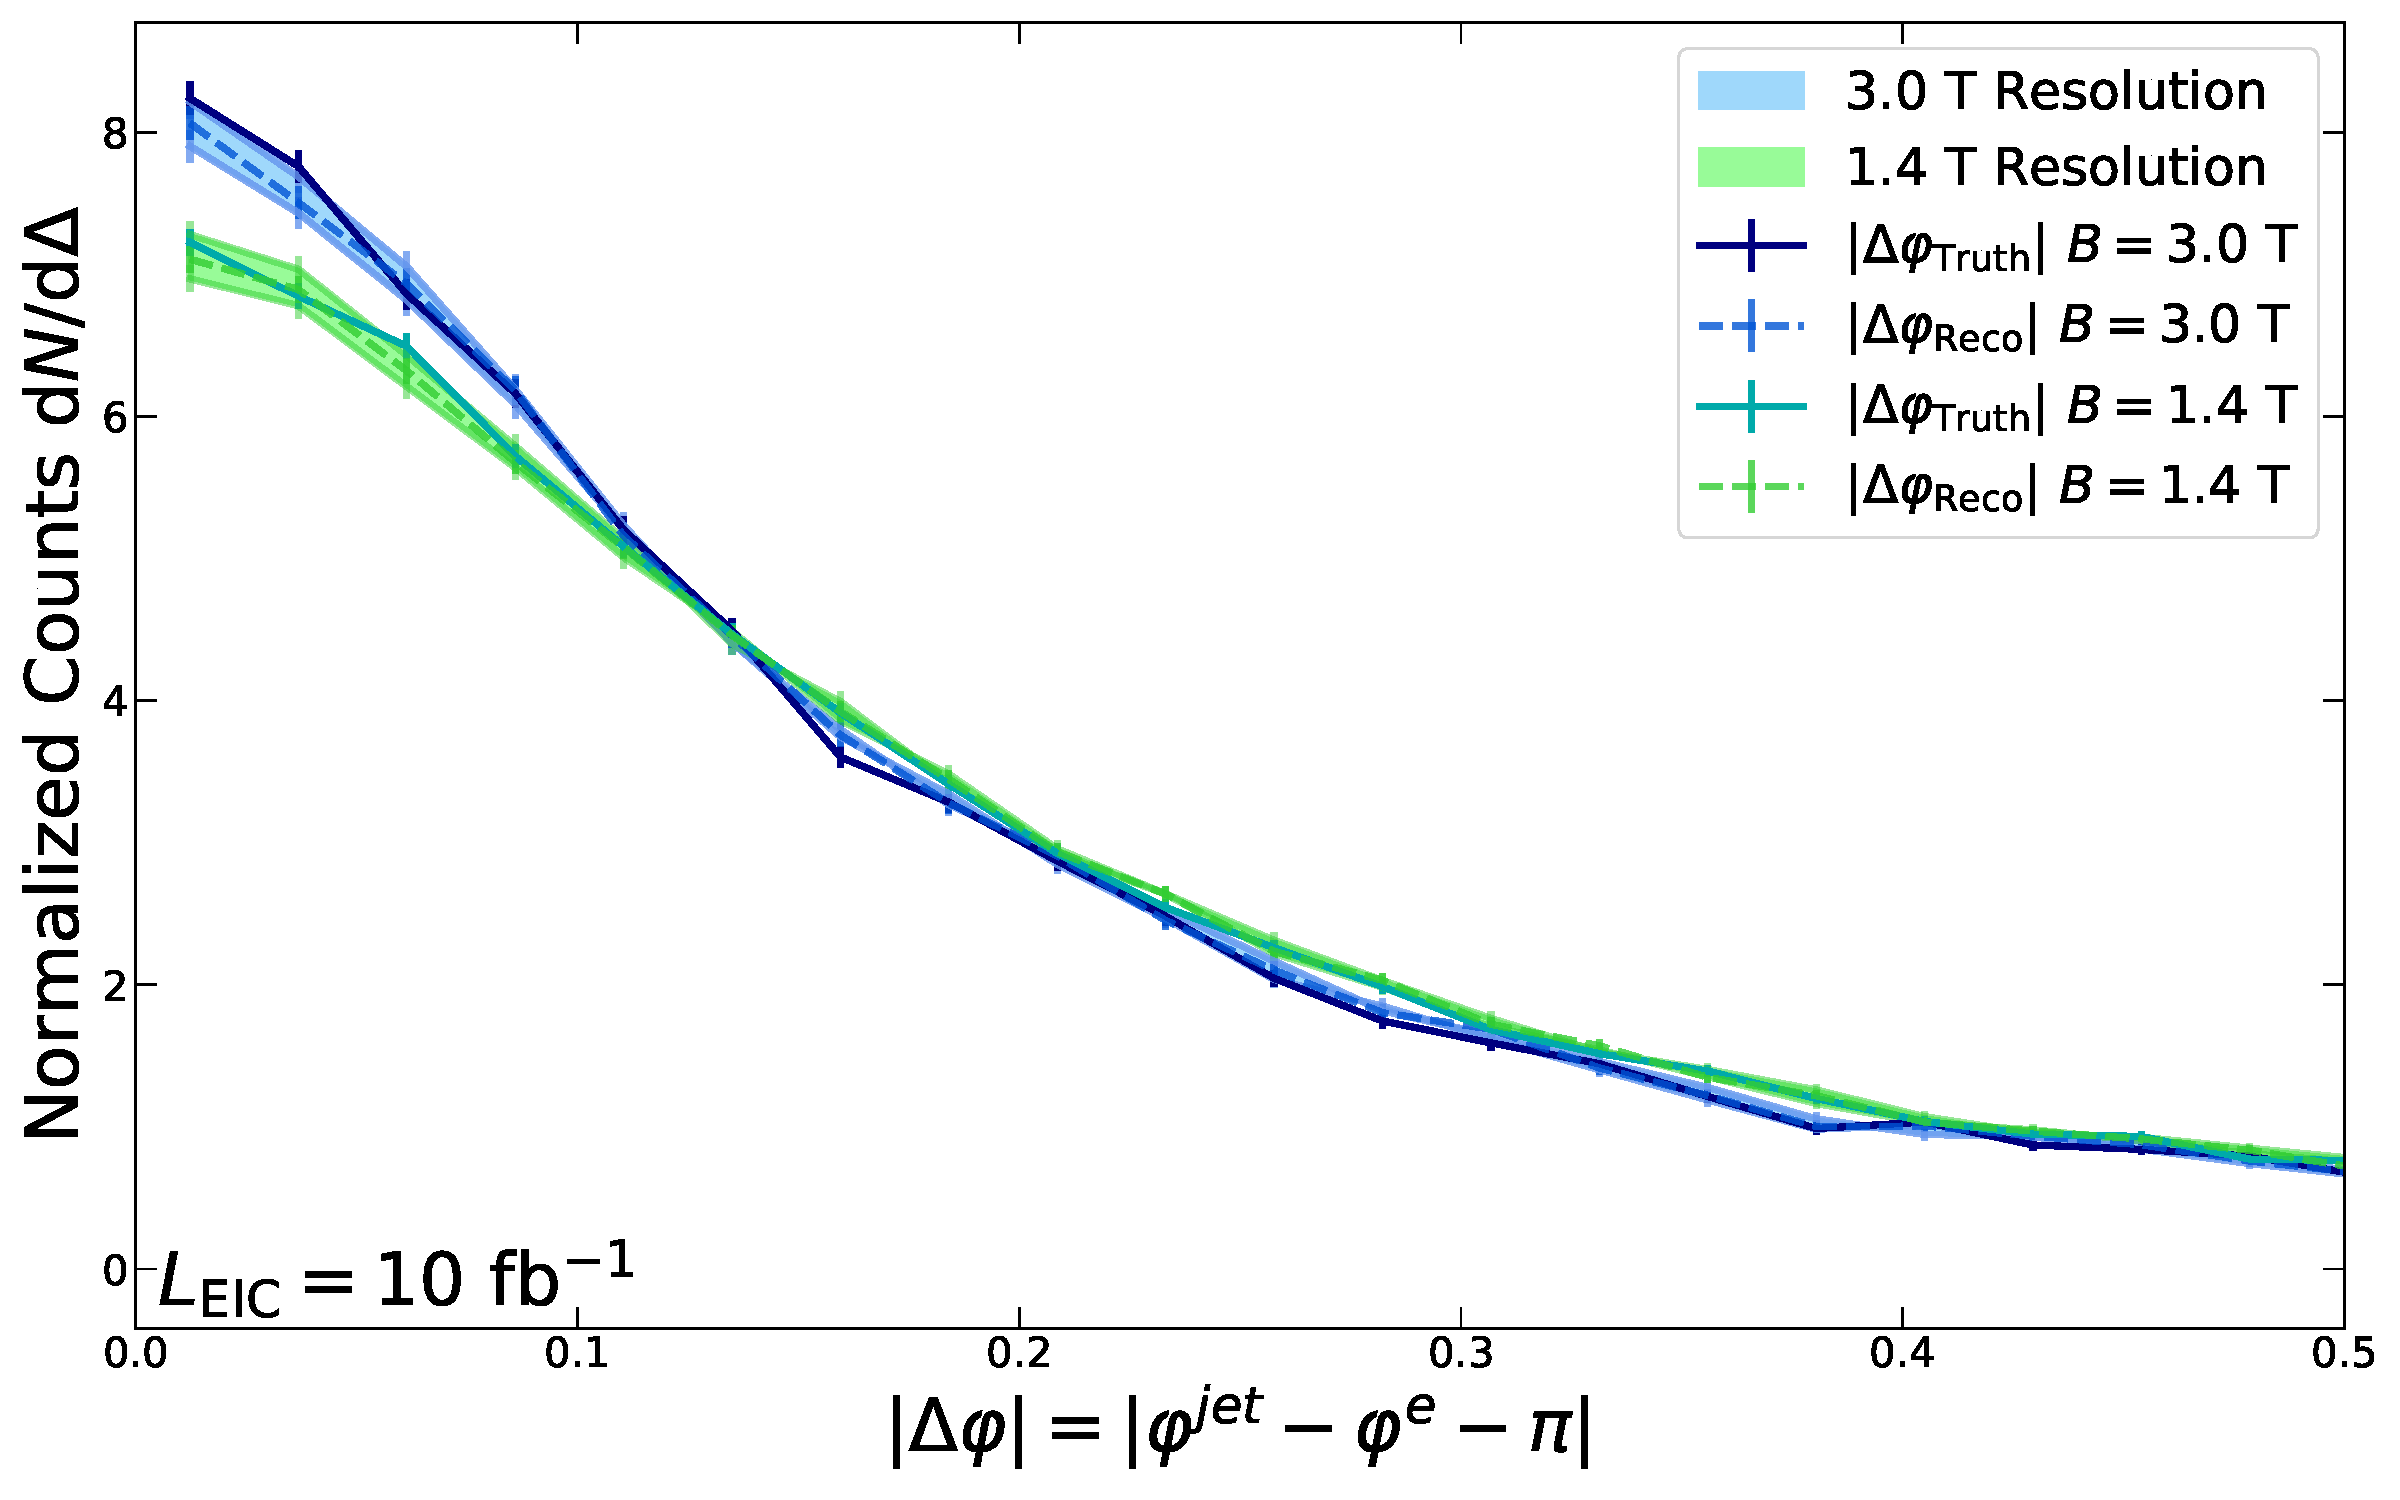
\includegraphics[width=0.99\textwidth]{EIC_Jets/azimuthal_correlations.pdf}
    \caption{Azimuthal correlation between the scattered electron and jets in $e$+$p$ collisions simulated with a 1.4 T and 3.0 T magnetic field. Solid lines display the correlation between particle-level scattered electron and jets. The dashed lines display the correlation between the reconstructed electron and reconstructed jets, with the shaded bands representing the uncertainty arising from the $\Delta\varphi$ resolution. The statistical error bars are scaled to reflect an expected luminosity of $L = 10\mathrm{fb}^{-1}$.}
    \label{fig:az_corr}
\end{figure}

Figure~\ref{fig:az_corr} shows full simulation results for the azimuthal difference between jets and the scattered electron, $|\varphi^\mathrm{jet} - \varphi^{e} - \pi|$ in a 1.4 and 3.0T magnetic field. Dashed lines display the correlation between the reconstructed scattered electron and charged jets both reconstructed with the all-silicon tracker. The darker solid lines show the correlation between the scattered truth electron and particle-level truth jets. The shaded bands centered on the reconstructed correlation reflect the estimated uncertainty arising from the $\Delta\varphi$ resolution, extracted by a fitting double Gaussian to $d\Delta\varphi$ distributions, where $d\Delta\varphi = (\Delta\varphi_\mathrm{truth}-\Delta\varphi_\mathrm{reco}/\Delta\varphi_\mathrm{truth}$. The band is obtained by varying the reconstructed $\Delta\varphi$ correlation by $\pm \sigma_\Delta\varphi$. The statistical error bars are scaled to reflect an expected luminosity of $L = 10\mathrm{fb}^{-1}$. Both the electron and jet momentum and azimuthal angle, $\varphi$, are reconstructed using the all-silicon tracker. The measurement on actual data, however, will likely implement an $E/P \approx 1.0$ selection on the electron. However, at the time of this simulation, a mature design of the backwards calorimeter responsible for measuring the electron's energy was not implemented. Instead, the electron truth energy was smeared by the backward calorimeter energy resolution of $\sigma(E)/E\approx 2\%\sqrt{E}\otimes (1-3)\%$ described in the EIC yellow report of \cite{Khalek2021}.

%The figure shows a peak at zero as expected from LO DIS where the electron and jet are emitted back-to-back. In the limit that the transverse momentum imbalance, $p_\mathrm{T}^e / p_\mathrm{T}^{jet}$, is much smaller than the electron transverse momentum, this observable can provide clean access to the quark TMD PDF and the Sivers effect in transversely polarized scatterings in $e$+$p$ collisions~\cite{Liu2019}.

%\begin{figure}[htbp]
%    \centering
%    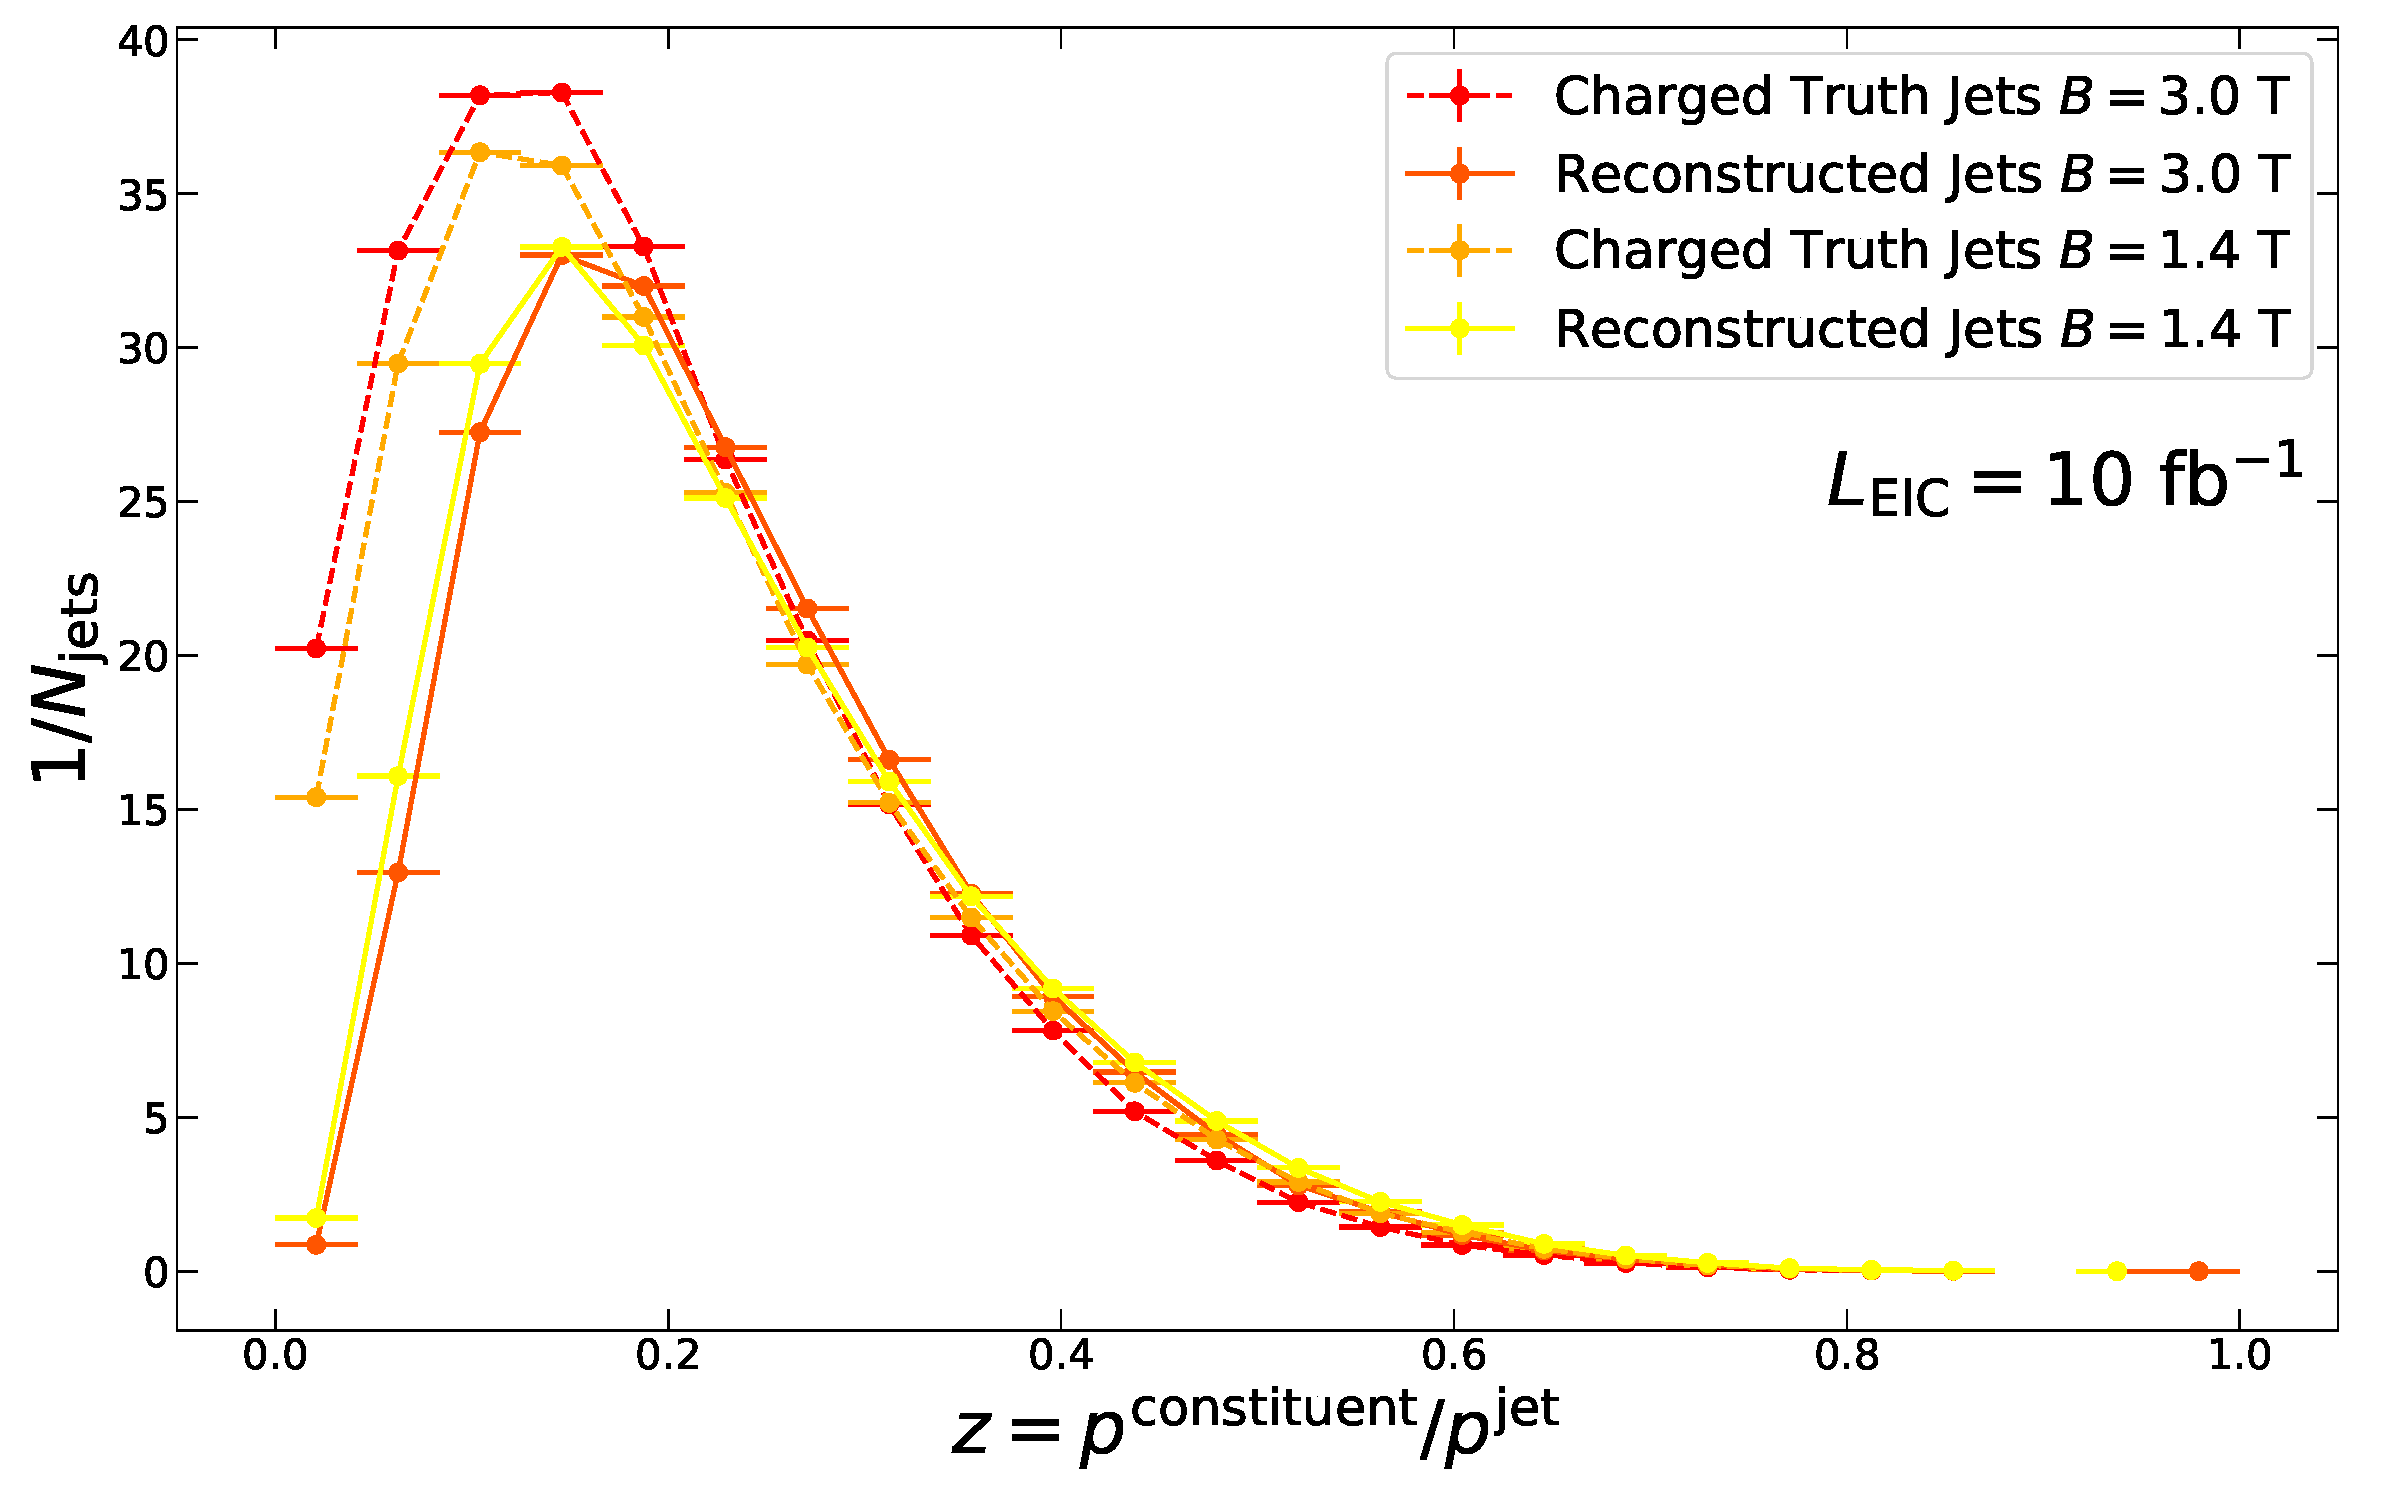
\includegraphics[height=0.4\textwidth,width=0.6\textwidth]{EIC_Jets/charged_jet_fragmentation.pdf}
%    \caption{Truth-level (dashed lines) and reconstructed-level (solid lines) charged jet fragmentation as a function of $z = p^\mathrm{constituent}/p^\mathrm{jet}$ in 1.4T and 3.0T magnetic fields. The statistical error bars are scaled to reflect an expected luminosity of $L = 10\mathrm{fb}^{-1}$.}
%    \label{fig:jet_frag}
%\end{figure}

%Figure \ref{fig:jet_frag} shows the particle-level (dashed lines) and reconstructed-level (solid lines) charged jet fragmentation functions in the two magnetic field configurations. Again, statistical error bars are scaled for an expected luminosity of $L = 10\mathrm{fb}^{-1}$. Measurements of the charged-jet fragmentation function in $e$+$p$ 
%%bvj is 
%should provide sensitivity to the process of hadron formation. 
%%bvj outside of a nucleus. 
%Comparisons of charged jet fragmentation functions measured in $e$+$p$ and $e$+A collisions can elucidate the effects of nuclear matter on the fragmentation process, and yield information on parton transport in a nuclear medium. For lower energy jets, which begin to fragment inside a nucleus in $e$+$A$ collisions, we can use the nucleus as a filter to probe hadronization. 


%The choice of magnetic field is shown to have little effect on both observables shown. While the different  magnetic fields result in different angular and momentum resolutions, that will in turn affect the the azimuthal correlation and fragmentation function measurements, the magnitude of these changes is quite small. For example, the momentum resolution for reconstructed jets with less than 1 missing constituent is approximately between 0.3\% and 0.45\% in a 3.0T magnetic field. In a 1.4T magnetic field, the momentum resolution ranges between 0.5\% and 0.75\%. This change in the momentum resolution of a few fractions of a percent is not expected to significantly impact the fragmentation function measurements. Similar reasoning applies to the differences in angular resolution and their effect on the electron-jet correlation measurements, however it should be noted that changes in the angular resolution will effect both the reconstructed jet as well as the reconstructed scattered electron. Nonetheless, the simulations indicate that the statistical precision of electron-jet correlations should be small enough to determine distinguish different values of $\hat{q}L$ shown in Fig.~\ref{fig:ql_corr}. However, direct comparisons to the model in \cite{Liu2019} will require dedicated e-A simulations.

